%%%%%%%%%%%%%%%%%%%%%%%%%%%%%%%%%%%%%%%%%%%%%%%%%%%%%%%%%%%%%%%%%%%%
%% I, the copyright holder of this work, release this work into the
%% public domain. This applies worldwide. In some countries this may
%% not be legally possible; if so: I grant anyone the right to use
%% this work for any purpose, without any conditions, unless such
%% conditions are required by law.
%%%%%%%%%%%%%%%%%%%%%%%%%%%%%%%%%%%%%%%%%%%%%%%%%%%%%%%%%%%%%%%%%%%%

\documentclass[
  digital, %% This option enables the default options for the
           %% digital version of a document. Replace with `printed`
           %% to enable the default options for the printed version
           %% of a document.
  oneside, %% This option enables double-sided typesetting. Use at
           %% least 120 g/m² paper to prevent show-through. Replace
           %% with `oneside` to use one-sided typesetting; use only
           %% if you don’t have access to a double-sided printer,
           %% or if one-sided typesetting is a formal requirement
           %% at your faculty. (twoside)
  table,   %% This option causes the coloring of tables. Replace
           %% with `notable` to restore plain LaTeX tables.
  lof,     %% This option prints the List of Figures. Replace with
           %% `nolof` to hide the List of Figures.
  lot,   %% This option prints the List of Tables. Replace with
           %% `nolot` to hide the List of Tables.
  %% More options are listed in the user guide at
  %% <http://mirrors.ctan.org/macros/latex/contrib/fithesis/guide/mu/fi.pdf>.
]{fithesis3}
%% The following section sets up the locales used in the thesis.
\usepackage[resetfonts]{cmap} %% We need to load the T2A font encoding
\usepackage[T1,T2A]{fontenc}  %% to use the Cyrillic fonts with Russian texts.
\usepackage{hyperref}
\usepackage[
  main=slovak, %% By using `czech` or `slovak` as the main locale
                %% instead of `english`, you can typeset the thesis
                %% in either Czech or Slovak, respectively.
  english, german, russian, czech, slovak %% The additional keys allow
]{babel}        %% foreign texts to be typeset as follows:
%%
%%   \begin{otherlanguage}{german}  ... \end{otherlanguage}
%%   \begin{otherlanguage}{russian} ... \end{otherlanguage}
%%   \begin{otherlanguage}{czech}   ... \end{otherlanguage}
%%   \begin{otherlanguage}{slovak}  ... \end{otherlanguage}
%%
%% For non-Latin scripts, it may be necessary to load additional
%% fonts:
\usepackage{paratype}
\def\textrussian#1{{\usefont{T2A}{PTSerif-TLF}{m}{rm}#1}}
%%
%% The following section sets up the metadata of the thesis.
\thesissetup{
    date          = \the\year/\the\month/\the\day,
    university    = mu,
    faculty       = fi,
    type          = mgr,
    author        = Bc. Peter Stanko,
    gender        = m,
    advisor       = {RNDr. Nikola Beneš\, Ph.D.},
    title         = {Kontr 2: Systém na automatizované spracovanie domácich úloh},
    keywords      = {Kontr 2, automatizovaná oprava domácich úloh, REST, Pracovník, KTDK, Portál, distribuovaný systém, Docker, webová služba, Stratus.FI},
    TeXkeywords   = {Kontr 2, automatizovaná oprava domácich úloh, REST, Pracovník, KTDK, Portál, distribuovaný systém, Docker, webová služba, Stratus.FI},
    abstract      = {Automatické spracovanie a vyhodnotenie funkcionality domácich úloh študentov zjednoduší prácu učiteľom a študentom poskytne spätnú väzbu takmer okamžite. Táto práca popisuje návrh nástroja na automatizované spracovanie domácich úloh -- Kontru 2, implementáciu jeho výkonnej časti, popis nasadenia systému a jeho testovacej prevádzky. },
    abstractEn = { Automatic homework processing and evaluation can improve the education process by providing fast feedback and reducing the worload on teachers. The system Kontr~2 designed in this thesis provides all the necessary tools for such automation. The thesis presents a detailed design and implementation of the execution part of the system, its deployment and results of its short operation period.},
    thanks        = {Na tomto mieste by som rád poďakoval vedúcemu práce RNDr. Nikolovi Benešovi, Ph.D. za ústretový prístup, odborné vedenie, užitočné rady a čas, ktorý mi venoval pri konzultáciách. Ďalej by som rád poďakoval všetkým, ktorí do projektu Kontr 2 prispeli alebo v~budúcnosti prispejú akýmkoľvek spôsobom, či už nahlásením chyby, prispením do kódovej základne, prípadne dobrou radou. V~neposlednom rade by som rád poďakoval rodine a priateľom za podporu pri písaní tejto práce.},
    bib           = sources.bib,
}
\usepackage{makeidx}      %% The `makeidx` package contains
\makeindex                %% helper commands for index typesetting.
%% These additional packages are used within the document:
\usepackage{paralist} %% Compact list environments
\usepackage{amsmath}  %% Mathematics
\usepackage{amsthm}
\usepackage{amsfonts}
\usepackage{url}      %% Hyperlinks
\usepackage{markdown} %% Lightweight markup
\usepackage{listings} %% Source code highlighting
\usepackage{titlesec}
\usepackage{graphicx}
\usepackage{braket}
\lstset{
  basicstyle      = \ttfamily,%
  identifierstyle = \color{black},%
  keywordstyle    = \color{blue},%
  keywordstyle    = {[2]\color{cyan}},%
  keywordstyle    = {[3]\color{olive}},%
  stringstyle     = \color{teal},%
  commentstyle    = \itshape\color{magenta}}
\usepackage{floatrow} %% Putting captions above tables
\floatsetup[table]{capposition=top}

\newcommand{\ssubsection}[1]{%
  \subsubsection[#1]{\raggedright\normalfont\itshape #1}}
  
\newcommand*{\fullref}[1]{\hyperref[{#1}]{\ref*{#1} \nameref*{#1}}}
\newcommand*{\footurl}[1]{\footnote{\url{#1}}}

\usepackage{csquotes}
\DeclareQuoteAlias{german}{slovak}

\begin{document}
\chapter*{Úvod}
\addcontentsline{toc}{chapter}{Úvod}

Už niekoľko rokov je na poradách predmetov \textit{PB071} a \textit{PB161} diskutovanou témou nevyhovujúci stav automatizácie opravy domácich úloh. V~súčasnosti používané riešenie je nedostatočné, kapacitne limitované a užívateľsky neprívetivé, čo bolo impulzom pre návrh a~implementáciu jeho náhrady, ktorú predstavuje táto práca.

Počas analýzy požiadaviek a návrhu systému bolo zistené, že nástroj je z~dôvodu jeho rozsiahlosti vhodné rozdeliť na viacero samostatných komponentov. Vďaka definovaným rozhraniam a využitiu technológii známych na Fakulte informatiky Masarykovej univerzity (ďalej FI MU) je možné časti systému spracovávať samostatne ako diplomové alebo bakalárske práce.

Projekt \textit{Kontr 2} má za cieľ stať sa úspešným následníkom nástroja \textit{Kontr}\cite{kontr} z~roku 2011, ktorý v~predmetoch \emph{Úvod do nízkoúrovňového programování (kód PB071)} a \emph{Programování v~jazyce C++ (kód PB161)} automatizuje prijímanie, spracovanie a hodnotenie domácich úloh. Nástroj vyučujúcim poskytuje aj webové rozhranie \textit{Kontr-logs}\cite{KontrWeb}, schopné zobrazovať jednotlivé odovzdania. Kontr má mnohé nedostatky, kvôli ktorým ho je vhodné nahradiť. Medzi najvýznamnejšie patria jeho nedostatočná škálovateľnosť, využívanie zastaralých technológií, neprehľadná kódová základňa a nezanedbateľné bezpečnostné chyby.

Nový projekt vzniká nezávisle na nástroji Kontr a snaží sa vyhnúť jeho chybám. Využitím moderných technológii a štrukturovaným návrhom umožňuje zapojenie širšieho okruhu vývojárov z~radov vyučujúcich i študentov. Projekt je vydaný ako projekt s~otvoreným zdrojovým kódom a definovanými procesmi ako do neho prispievať.

V~tejto práci je popísaná analýza požiadaviek na systém automatizovanej opravy domácich úloh Kontr 2, navrhnutá štruktúra systému a implementovaná jeho výkonná časť, ktorá poskytuje syntax a behové prostredie pre vykonávanie prispôsobiteľných testov. Dôležitou časťou práce bola identifikácia komponentov systému, určenie rozhraní a komunikácie medzi komponentmi, vymedzenie hraníc systému a jeho komunikácie ako celku s~externými entitami (Databáza, Dodávateľ identít, Informačný systém Masarykovej univerzity (ďalej IS MU)).

Vytvorený systém umožňuje automatizované spracovanie študentských riešení programovacích domácich úloh v~širokom spektre predmetov s~možnosťou prispôsobenia ich špecifickým požiadavkám. Systém poskytuje rozhranie na prijímanie študentských odovzdaní, umožňuje ich spracovanie automatizovanými nástrojmi kontroly kvality a v~štrukturovanej forme sprístupňuje výsledky vyučujúcim aj študentom.

Práca sa skladá zo štyroch logických častí. Prvá časť práce sa venuje analýze požiadaviek, zavádza pojmy z~problémovej domény a prestavuje problematiku automatizovaného spracovania úloh. Druhá časť práce sa zaoberá návrhom systému, popisu konceptov použitých v~práci, špecifikáciou rozhraní a komunikácie jednotlivých komponent. Tretia časť obsahuje popis implementácie častí systému a použitých technológii. Štvrtá časť sa venuje nasadeniu systému, testovacej prevádzke a spôsobom dodania jednotlivých závislostí a častí systému. 


\chapter{Automatizovaná oprava domácich úloh}

Na FI MU je vyučovaných mnoho programovacích predmetov, súčasťou ktorých sú programátorské úlohy, ktoré študent vypracováva doma alebo na cvičení. Študent podľa zadania vytvára riešenie vo forme zdrojového kódu v~predpísanom programovacom jazyku. Vypracovania sú hodnotené na základe ich funkčnosti (miery naplnenia zadania), programátorského štýlu, prípadne ďalších kritérií špecifických pre predmet. 

Proces hodnotenia prebieha spravidla v~troch krokoch:
\begin{enumerate}
    \item Študent svoje vypracované riešenie sprístupní hodnotiteľovi (človeku alebo systému). Najviac využívanými metódami odovzdania na FI MU sú nahranie súborov do \textit{Odevzdávárny}\footurl{https://is.muni.cz/napoveda/ucitel/odevzdavarny} IS MU alebo sprístupnenie kódu pomocou systému na správu verzií, napr. \textit{Git}\footurl{https://git-scm.com} alebo \textit{SVN}\footurl{https://subversion.apache.org/}. 
    \item V~definovanom termíne opravujúci získa študentovo odovzdanie, ohodnotí mieru naplnenia zadania, programátorského štýlu, efektívnosti a iných kritérií špecifických pre predmet. 
    \item Hodnotenie je prevedené na body či slovné zhrnutie a uložené v~IS MU, typicky pomocou zápisu do \emph{Poznámkových blokov} IS~MU\footurl{https://is.muni.cz/napoveda/ucitel/bloky}.
\end{enumerate}

Všetky tri kroky tohoto procesu je možné do určitej miery automatizovať a odbremeniť tak vyučujúcich. Pre automatizáciu je možné využiť jednoduché porovnávanie výstupu, rámce a knižnice pre jednotkové testy (napr. \emph{JUnit}\footnote{\url{https://junit.org/junit5/}}, \emph{Catch2}\footnote{\url{https://github.com/catchorg/Catch2}}), nástroje na kontrolu formátovania (\emph{clang-format}\footnote{\url{https://clang.llvm.org/docs/ClangFormat.html}}, \textit{pylint}\footnote{\url{https://www.pylint.org/}}), programátorského štýlu (\textit{clang-tidy\footnote{\url{http://clang.llvm.org/extra/clang-tidy/}} a clang-format}) alebo zložitosti kódu (\textit{Rubocop}\footnote{\url{https://github.com/rubocop-hq/rubocop}}, \textit{cppcheck}\footurl{http://cppcheck.sourceforge.net/}). Ich hlavnými výhodami sú rýchlosť a jednotnosť (v~hodnotení aj vo výstupe), ktorá garantuje rovnaké podmienky pre všetkých študentov. Študentom je tak možné rýchlejšie poskytnúť spätnú väzbu na ich riešenia, prípadne ich nasmerovať na príčinu zlyhania. Rovnako sa znižuje aj miera nejednotnosti hodnotenia, ktorá je často prítomná ak je hlavným hodnotiteľom človek.

Minimalizácia či odstránenie ľudského faktoru z~procesu opravy úloh prináša časovú úsporu študentom i vyučujúcim, zjednocuje podmienky hodnotenia úloh, prináša jasný, kvantifikovateľný výstup a zmenšuje priestor pre chyby. Automatická kontrola odovzdaní ale nemôže kontrolu človekom plne nahradiť, zapojenie opravujúceho je v~procese výuky jednou z~nevyhnutných podmienok. Študentov je potrebné pripraviť aj na neskoršiu programátorskú prax, ktorej súčasťou je kontrola kódu zo strany spolupracovníkov\cite{code_reviews_atlassian}. Podobne ako zákony nie je možné vykladať na súde strojovo ale je potrebný sudca, tak aj pri opravovaní úloh je potrebný ľudský zásah na rozsiahlu a personalizovanú spätnú väzbu\cite{code-feedback}. Cieľom automatizácie je človeku prácu zjednodušiť a študentom poskytnúť spätnú väzbu rýchlejšie.

Tieto dôvody boli dostatočným faktorom pre vytvorenie nového nástroja pre automatizáciu procesu odovzdávania úloh, ktorý môže byť veľkým prínosom pre mnoho programovacích predmetov vyučovaných na FI MU. Počet študentov prijímaných na FI MU stále stúpa a zefektívnenie práce vyučujúcich je preto vhodným spôsobom, ako udržať kvalitu štúdia na dobrej úrovni.

Aby bol systém na automatickú opravu domácich úloh použiteľný, musí byť pri jeho návrhu a implementácií kladený dôraz na niekoľko významných vlastností\cite{obrien-attributes-soa}:

\begin{itemize}
    \item \textit{Bezpečnosť} - Žiaden používateľ by nemal byť schopný čítať alebo meniť informácie ku ktorým nemá mať prístup. Zmeny v~systéme musia byť zaznamenávané, aktéri identifikovateľní. Činnosť bežných používateľov nesmie ohroziť stabilitu a dostupnosť systému.
    \item \textit{Škálovateľnosť} - V~prípade potreby je možné zvýšiť priepustnosť systému pridaním ďalších zdrojov.
    \item \textit{Robustnosť} - V~prípade výpadku je možné systém obnoviť, predovšetkým je potrebné zaručiť integritu používateľských dát.  
    \item \textit{Prenositeľnosť} - Systém alebo jeho časti je možné nasadiť na rôznych platformách alebo verziách operačného systému.
    \item \textit{Ľahkú rozšíriteľnosť} - Do systému je možné bez veľkých zásahov pridať novú funkcionalitu alebo pozmeniť už existujúcu.
    \item \textit{Integrácia} - Systém je možné napojiť na služby poskytované FI~MU a~IS~MU.
\end{itemize}

Systém s~výraznými nedostatkami v~ktorejkoľvek z~týchto kategórií je v~praxi nepoužiteľný. Preto boli tieto kritériá základom ďalšieho rozhodovania a hlavným dôvodom zamietnutia už existujúcich nástrojov pre potreby FI MU. Napriek tomu je podstatné uviesť existujúce riešenia a predstaviť dôvody implementácie vlastného projektu.

\section{Existujúce automatizačné nástroje}

V~súčasnosti existujú viaceré nástroje na automatizovanú opravu domácich úloh, od tých s~otvoreným zdrojovým kódom, napríklad  \textit{Submitty}\footnote{https://submitty.org/}, ktoré je možné nasadiť a používať na vlastnej infraštruktúre, až po celé komerčné cloudové riešenia \textit{Vocareum}\footnote{https://www.vocareum.com/} alebo \textit{GradeScope}\footnote{https://www.gradescope.com/}, ktoré sú platené. Na FI MU tiež existuje nástroj Kontr, umožňujúci automatizáciu odovzdania a kontroly domácich úloh.

Plateným nástrojom nasadeným u~externých dodávateľov v~\emph{cloude}, som sa chcel od začiatku vyhnúť. Prichádzajú s~nimi rôzne problémy ako nemožné alebo obtiažne prispôsobenie, komplikované licenčné podmienky, nedostatočná transparentnosť a kontrola, možné komplikácie s~legislatívou a nezanedbateľný finančný faktor.

Riešenie s~otvoreným zdrojovým kódom nedosahovalo dostatočnú mieru rozšíriteľnosti pre špecifické požiadavky niektorých predmetov vyučovaných na fakulte. Okrem toho bolo postavené na jazykoch, ktoré sa na fakulte nevyučujú \emph{(PHP)}, čo by pravdepodobne znamenalo nízku mieru zapojenia študentov a vyučujúcich do vývoja nástroja.

Celkovo existujúce nástroje zaostávali v~ohľadoch flexibility (nízkymi možnosťami rozšírenia, platformovou závislosťou, nedostatočnou úrovňou oprávnení) alebo obsahovali nepotrebnú funkcionalitu.

Po preštudovaní dostupných nástrojov a zvážení ich výhod a nevýhod som dospel k~záveru, že vlastná implementácia je najlepšou cestou, nad ktorou bude mať fakulta a jednotlivé predmety kontrolu. Bude možné ju upraviť a prispôsobiť podľa dodatočných požiadaviek. Ďalšou výhodou je jednoduchá integrácia so službami využívanými a poskytovanými na FI MU.

\subsection{CI/CD Nástroje}

\emph{Priebežná integrácia (Continous Integration, CI)}\cite{mfowler-ci} je v~súčasnosti jedným z~hlavných princípov využívaných pri vývoji softvéru. Ide o~spúšťanie automatizovaných testov nad každou novou verziou kódu, čo umožňuje väčšiu mieru kontroly spoľahlivosti, rýchle odhaľovanie chýb a pri správne nastavených procesoch čiastočnú ochranu pred zavedením defektu alebo znefunkčnením kódovej základne. Dôvera vo fungovanie systému po každej zmene je základom implementácie \emph{priebežného doručovania (Continuous Delivery, CD)}\cite{continous-delivery}. Rýchle nasadenie otestovaných zmien umožňuje inkrementálny vývoj systému a odstraňuje možnosť zanášania chýb či nekonzistencií spôsobených ľudským faktorom. Medzi najširšie používané nástroje CI/CD patria \textit{Jenkins}\footnote{\url{https://jenkins.io}}, \textit{Travis}\footnote{\url{https://travis-ci.org/}} a \textit{GitLab-CI}\footnote{\url{https://about.gitlab.com/product/continuous-integration/}}. 

Spomenuté nástroje by bolo možné využiť pri automatickej oprave domácich úloh, pretože ich princíp sa do určitej miery prekrýva s~myšlienkou kontroly domácich úloh. Hlavnou úlohou CI/CD nástrojov je spúšťanie tzv. \emph{jobov} na základe notifikácií, prijímaných väčšinou vo forme \emph{webhooku}. Job je súbor akcií, ktoré sa majú vykonať pri prijatí definovanej notifikácie. Typicky ide o~skript v~nejakom programovacom jazyku, ktorý umožňuje definíciu požadovaných akcií. Využívané sú predovšetkým na spúšťanie automatizovaných testov v~systémoch na správu \emph{git repozitárov} ako napríklad \emph{GitLab}\footnote{\url{https://gitlab.com}} alebo \emph{GitHub}\footnote{\url{https://github.com}}, spolu s~prípravou či nasadením do určitého behového prostredia.  

Hlavnou výhodou CI/CD nástrojov je, že väčšina programátorov sa s~nimi stretne v~praxi a neboli by pre nich úplnou novinkou. Korektná konfigurácia týchto nástrojov je ale pre účely automatizovanej opravy domácich úloh pomerne komplikovaná. V~nástrojoch totiž nie sú dostatočne oddelené úrovne oprávnení a nie je jednoduché ich nastaviť tak, aby sa neoprávnení používatelia nedostali k~citlivým dátam. Nástroje by bolo potrebné obaliť vlastnými autorizačnými mechanizmami, ktoré by rešpektovali štruktúru kurzov a úloh a dokázali riadiť prístup k~výsledkom spracovaní podľa roly používateľa v~kurze.

Druhým problémom je komplikovaný popis zložitejších testovacích scenárov, ktorý by pre zadávajúceho domácej úlohy znamenal netriviálnu záťaž. Konfigurácia nástrojov totiž využíva vlastné DSL (Jenkins) alebo značkovací jazyk (GitLab CI), v~ktorých je zápis rozsiahlych scenárov ťažko čitateľný a spravovateľný. Využitie tzv. \textit{scripted pipelines} systému Jenkins by vyžadovalo definíciu samostatnej knižnice pomocou jazyka Groovy, ktorý sa na FI MU nevyučuje.

Treťou problematickou oblasťou je komplikovaný proces odovzdania riešenia, ktorý by od študentov vyžadoval komplexnejšie znalosti verzovacieho systému a nebol by vhodný pre úvodné kurzy programovania vyučované na fakulte.

\subsection{Nástroj Kontr}

Na FI MU je v~súčastnosti v~predmetoch PB071 a PB161 používaný nástroj Kontr, ktorý bol založený v~roku 2011 RNDr. Šimonom Tóthom a v~priebehu rokov sa na jeho vývoji podieľalo mnoho ľudí s~rôznymi programovacími návykmi. Implementovaný je v~jazyku \emph{Perl}\footnote{\url{https://dev.perl.org/perl5/}}.

Prvotná implementácia vznikla v~pomerne krátkom čase a následne sa na ňu nabaľovali rôzne rozšírenia a záplaty. Systém trpí niekoľkými zásadnými chybami v~návrhu, má nedostatočnú dokumentáciu a miestami nečitateľný kód. Všetky tieto vady majú za následok nedostatky nástroja v~rozšíriteľnosti, prenositeľnosti a bezpečnosti. O~správu nástroja a jeho úpravy sa v~súčasnosti stará Mgr. Roman Lacko. 

Pomocou nástroja Kontr študent odovzdáva vypracovanie svojej úlohy spustením skriptu \texttt{odevzdavam}. Ten vytvorí nový súbor v~špeciálnom priečinku s~informáciou, pre ktorý predmet a pre ktorú úlohu bolo odovzdanie vytvorené. Následne sa v~päťminútových intervaloch spúšťa \textit{Cron job}\footnote{\url{http://pubs.opengroup.org/onlinepubs/9699919799/}}, ktorý prejde adresár a postupne spustí vykonávanie jednotlivých odovzdaní. Odovzdanie je spustené s~právami užívateľa \emph{kontr} definovaného vo fakultnej databáze používateľov. Súčasťou spracovania je stiahnutie študentovho vypracovania z~repozitáru na fakultnom GitLabe. Kontr si obsah repozitára uchováva dlhodobo (až do jeho manuálneho zmazania) a pre aktualizáciu vykonáva príkaz \texttt{git pull}\footurl{https://git-scm.com/docs/git-pull}. 

Testovanie je vykonávané pomocou vlastného testovacieho rámca implementovaného v~jazyku Perl, ktorý je súčasťou samotného nástroja. Testovacie scenáre pre všetky domáce úlohy sú dodávané v~separátnom repozitári. Kontr po dokončení testovacieho procesu odošle email s~výsledkami študentovi aj jeho opravujúcemu pre danú domácu úlohu. Aktuálna verzia dokáže komunikovať s~rozhraním Poznámkových blokov IS MU\footurl{https://is.muni.cz/napoveda/technicka/bloky_api}, do ktorých zapisuje výsledky testov aj s~bodovým hodnotením.

Výsledky automatizovaného testovania je možné prezerať vo webovom rozhraní \textit{Kontr-logs}\cite{KontrWeb} určenom pre opravujúcich domácich úloh. Je v~ňom možné zobraziť výsledky jednotlivých testov, výstupy behu testov a samotné odovzdania študentov. Pomocou nástroja je možné porovnávať zdrojové kódy pre jednotlivé odovzdania a znova otestovať už existujúce odovzdanie. 

Napriek svojej užitočnosti je Kontr nevhodný na ďalšie používanie predovšetkým kvôli nasledujúcim vadám:
\begin{itemize}
    \item \emph{monolitická architektúra}: celý systém je jeden celok a chyba jednej z~jeho častí môže spôsobiť zlyhanie celého nástroja. Silná previazanosť súčastí nástroja zhoršuje jeho rozšíriteľnosť.
    \item \emph{jazyk Perl}: na FI MU nie je vyučovaný, preto nie je veľa ľudí ktorí by mohli prispievať do jeho kódovej základne.
    \item \emph{neprehľadná kódová základňa}: v~snahe minimálne zasahovať do jadra nástroja rozšírenie Kontru neprebieha zmenou v~jeho kódovej základni, ale sadou podporných skriptov. Z~dlhodobého hľadiska ide o~neudržateľné riešenie.
    \item\emph{bezpečnostné vady}: Odovzdaný kód sa môže dostať aj k~informáciám, ku ktorým by nemal mať prístup, dokonca by mohol zmazať alebo poškodiť domovský adresár užívateľa \textit{kontr}.
    \item \emph{neprenositeľnosť}: Kontr je pevne zviazaný s~fakultnou infraštruktúrou natoľko, že ho nie je možné spustiť mimo stroja \textit{Aisa}\footnote{\url{https://www.fi.muni.cz/tech/unix/aisa.html.cs}}. Dôsledky tohoto obmedzenia sú predovšetkým nízka škálovateľnosť z~dlhodobého (nedostatočné diskové kvóty na skladovanie odovzdaní) i krátkodobého hľadiska (vysoké vyťaženie stroja pred koncom odovzdávania) a závislosť na danej platforme.
    \item \emph{nedostatočné oddelenie oprávnení}: Aktuálna architektúra predpokladá striktné oddelenie role \emph{študent} a \emph{učiteľ} pre všetky predmety. Preto ak je užívateľ učiteľom jedného predmetu, má učiteľské práva pre všetky predmety.
\end{itemize}



\chapter{Analýza požiadaviek na Kontr 2}

Pri vývoji nového softvéru je analýza požiadaviek základom, z~ktorého vyplýva užitočný návrh a implementácia zodpovedajúca zámeru projektu. Keďže chyby v~požiadavkách na systém sa typicky prejavujú až v~jeho prevádzke, je kritické tejto fáze venovať najviac pozornosti. 

\emph{Funkčné} i \emph{nefunkčné požiadavky} na nový systém vyplývajú predovšetkým z~dvoch zdrojov: odhalených nedostatkov nástroja Kontr a od vyučujúcich rôznych programovacích predmetov na FI MU, ktorí by mali záujem Kontr 2 v~budúcnosti využívať. Oba zdroje sú rovnako podstatné, aby bol nový nástroj využiteľný v~praxi. Okrem toho je nutné v~dostatočnej miere dbať na kritériá stanovené v~predchádzajúcej kapitole.

Najviac detailne projekt zohľadňuje požiadavky predmetov \emph{PB071 (C)} a \emph{PB161 (C++)}, ktoré využívajú starý Kontr a sú primárnymi kandidátmi na budúcich používateľov Kontru 2. Všeobecné požiadavky predmetov vyučujúcich predmetov Programovanie v~jazykoch \emph{Java}, \emph{Python}, \emph{Ruby} alebo\emph{C\#} boli spracované menej detailne a systém bude pred použitím v~týchto predmetoch nutné rozšíriť o~podporu daných jazykov a nástrojov. 

\section{Funkčné požiadavky}

Funkčné požiadavky definujú požadované správanie systému. Ide o~detailnejšie rozpracovanie myšlienky automatickej opravy domácich úloh na čiastkové procesy, ktoré umožňuje presnejšie premietnutie výukového procesu FI MU do nového nástroja. Pre prehľadnosť sú požiadavky uvedené v~samostatných kategóriách napriek tomu, že kategórie sú navzájom prepojené.

\subsection{Hlavný prípad použitia}

Systém Kontr 2 je určený na automatizáciu procesu opravy domácich úloh. V~kontexte výuky na FI MU pojem \textit{odovzdanie} odkazuje na jednu inštanciu riešenia zadania domácej úlohy. Typicky ide o~funkčný kód, ktorý je základom pre hodnotenie študenta v~danej úlohe. V~programovacích predmetoch na FI MU je často podmienkou úspešného ukončenia predmetu vyriešenie celého súboru úloh, zadávaného počas semestra. Úlohy majú za cieľ overiť a precvičiť nadobudnuté schopnosti študentov v~preberaných oblastiach. 

Hlavným prípadom užitia systému je poskytnúť nástroj pre automatizované spracovanie \emph{odovzdania}. Odovzdanie vytvára študent pre \emph{domácu úlohu (projekt)}, ktorá bola zadaná v~študovanom \emph{predmete}. Nad odovzdaním je spustená definovaná sada testovacích scenárov, ktoré majú za cieľ otestovať funkcionalitu. Výsledky testovania sú následne zaznamenané a vyhodnotené. O~dostupnosti výsledkov je notifikovaný \emph{študent} aj \emph{opravujúci} (väčšinou učiteľ) pridelený danému študentovi pre danú úlohu.

Proces automatizovanej opravy študentských riešení v~minimálnej podobe obsahuje v~časovej následnosti tieto kroky:
\begin{enumerate}
    \item Študent sa prihlási do systému.
    \item Študent si vyberie predmet a úlohu.
    \item Študent vytvorí odovzdanie s~dodatočnými parametrami potrebnými pre spracovanie odovzdania a jeho správne zaradenie.
    \item Systém odovzdanie uloží a pripraví prostredie pre jeho spracovanie.
    \item Systém spustí automatizované spracovanie odovzdania -- testovacie scenáre.
    \item Systém vyhodnotí výsledky testov a výsledky trvalo uloží.
    \item Systém notifikuje autora odovzdania a jeho opravujúceho o~výsledkoch.
    \item Študent si môže prezrieť svoje odovzdanie, čiastočné výsledky spracovania a hodnotenie v~systéme.
    \item Učiteľ si môže prezrieť študentovo odovzdanie a pridať slovné hodnotenie v~podobe komentárov. 
\end{enumerate}

Zjednodušený priebeh takejto opravy je spolu so zodpovedajúcimi nahradenými krokmi manuálnej opravy znázornený v~diagrame \ref{fig:eval-process}.

\begin{figure}[!ht]
  \begin{center}
    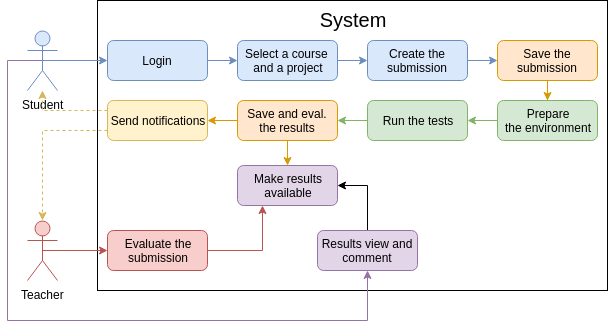
\includegraphics[width=\textwidth]{imgs/eval-process.png}
  \end{center}
    \caption{Diagram procesu odovzdania}
    \label{fig:eval-process}
\end{figure}

\subsection{Automatické spracovanie odovzdania}

Pri spracovaní študentského riešenia úlohy je potrebné, aby systém dokázal prijímať odovzdania z~rôznych zdrojov (predovšetkým zo systému \emph{Git}), dokázal ich dlhodobo uložiť, spracovať ich a sprístupniť výsledky spracovania študentom aj vyučujúcim. Popis modelovaného procesu a zasadenie entity \textit{odovzdanie} do kontextu je detailne rozpracované v~bakalárskej práci Bc. Barbory Kompišovej\cite{kontr-portal}.

Spracovanie odovzdaní je potrebné \emph{časovo plánovať}. Študent má mať možnosť svoje odovzdanie zrušiť v~presne definovanom časovom intervale, pred tým, než sa odovzdanie začne spracovávať. Rovnako je potrebné zabrániť zneužívaniu nástroja príliš častým odovzdávaním -- študent má preto povolený len obmedzený počet odovzdaní za určitý časový interval, čím je možné do určitej miery zabrániť preťaženiu nástroja.

Je vhodné aby Kontr 2 umožňoval prezeranie, hodnotenie a porovnávanie odovzdaní vyučujúcimi, ako to umožňuje už existujúci nástroj Kontr.
Študenti majú sprístupnené svoje vlastné odovzdania, ktoré si môžu prezerať, spolu s~prípadnými komentármi a hodnotením vyučujúceho. 

Pred študentmi je potrebné skryť časti výstupu testov, aby sa predišlo "`implementáciám podľa testov"' namiesto implementácií podľa zadania úlohy. Možnosť práce s~odovzdaním priamo cez nástroj Kontr~2 (prezeranie zdrojových kódov odovzdaní, ich komentovanie) zrýchli prácu opravujúcich, pretože nebudú musieť manuálne získavať odovzdania a výsledky automatického spracovania. 

V~budúcnosti je plánované rozšíriť systém o~automatické zadávanie hodnotenia do Poznámkových blokov IS MU. Pre zjednodušenie práce so systémom je tiež prínosné rozosielať študentom i vyučujúcim notifikácie o~spracovaní odovzdaní a ich výsledkoch. 

\subsection{Užívatelia a logické členenie}

Pre použitie systému Kontr 2 v~reálnej prevádzke je potrebné zabezpečiť správu \emph{používateľských účtov} a \emph{prístupových práv}, aby sa predišlo únikom informácií o~úlohách a odovzdaniach. Zásadnú úlohu má autentizácia používateľov, ktorú je možné zabezpečiť integráciou s~existujúcimi autentizačnými mechanizmami na FI~MU. Spojenie s~fakultnými nástrojmi umožní získanie dodatočných informácií o~užívateľoch a podrobnejšiu kontrolu používateľských oprávnení.

Autorizácia používateľov musí zodpovedať ich právam v~modelovanom procese výuky. Predovšetkým je nutné oprávnenia spravovať na úrovni predmetov, nie celého systému, ako s~nimi pracuje súčasný Kontr. Jeden užívateľ môže byť počas jedného semestra vyučujúci jedného predmetu a študent v~inom, čo mu v~každom predmete pripisuje inú množinu oprávnení. Vzhľadom na rozdielnu organizačnú štruktúru študovaných predmetov je vhodné umožniť jemnejšie oddelenie právomocí než len dve základné roly (študent/vyučujúci), čím je možné modelovať napríklad roly \emph{pomocník} či \emph{vlastník predmetu (prednášajúci)}, ktoré lepšie zodpovedajú realite.

Rôzne predmety môžu mať rôzne požiadavky na priradenie rolí alebo oprávnení pre jednotlivých užívateľov. Napríklad pre predmet PB161 bolo potrebné umožniť prideľovanie vyučujúceho (opravujúceho) študentovi pre každú úlohu osobitne.

\subsection{Požiadavky na správu a komunikáciu}

Administrácia systému prebieha na dvoch úrovniach -- vyučujúcimi, ktorí sú zodpovední za určitý predmet, a systémovým administrátorom, ktorý prevádzkuje a monitoruje všetky komponenty systému. 

Vyučujúci predmetu má v~rámci daného predmetu predovšetkým možnosť spravovať oprávnenia používateľov a jednotlivé úlohy. Principiálne ide len o~konfiguráciu malej množiny funkcionality systému, špecifickej pre daný predmet. Pre pohodlnú prácu je však výhodné sprístupniť potrebné administratívne úkony v~rozhraní systému, aby ich bolo možné vykonávať automatizovane.

Správa celého systému zahŕňa predovšetkým nasadenie a monitorovanie všetkých jeho súčastí. Je potrebné mať možnosť komponenty systému spravovať vzdialene pomocou administrátorského rozhrania, vyžadujúceho špeciálny typ používateľa a autentizáciu na úrovni každej samostatnej súčasti systému.

Bežným používateľom je vhodné pre jednoduché používanie funkcionalitu systému sprístupniť pomocou grafického rozhrania. Medzi jednotlivými komponentmi je potrebné umiestniť strojovo ľahko spracovateľné rozhrania. Rozhrania umožňujú nízku previazanosť komponentov, ich škálovateľnosť (napr. zvýšením počtu replík), využitie rôznych konkrétnych implementácií a prípadné nahradenie celého komponentu.

\section{Nefunkčné požiadavky}

Okrem funkcionality je pre systém potrebné špecifikovať aj požiadavky a obmedzenia na prevádzku systému, nazývané tiež nefunkčné požiadavky. Definujú podmienky prevádzky systému ako celku v~niekoľkých oblastiach. Ich cieľom je zaručiť kvalitu prevádzky aj procesu vývoja výsledného produktu.

\subsection{Bezpečnosť}
Bezpečnosť systému je jednou zo základných požiadaviek a zasahuje do mnohých jeho častí.

Jedným aspektom je kontrola prístupu používateľov k~údajom v~systéme, ktorú je potrebné zabezpečiť pomocou autentizačných a autorizačných mechanizmov, detailnejšie popísaných v~časti \fullref{impl-portal}.

Druhou časťou bezpečnosti systému je nutnosť ochrany proti externým útočníkom. Predovšetkým je nutné zabezpečiť, aby všetka komunikácia vonkajšieho sveta so systémom prebiehala šifrovane, sanitizovať vstupy a znížiť dopad útokov typu DOS\footnote{\url{https://www.us-cert.gov/ncas/tips/ST04-015}}. 

Tretím bodom je zabezpečenie izolovaného prostredia spúšťania odovzdaní študentov, ktoré odstráni nebezpečenstvo ovplyvňovania systému, interferencií medzi odovzdaniami, úniku a poškodeniu či neoprávnenej úpravy dát (napr. testov k~danej úlohe).

Pre správu a audit prevádzky systému je vhodným základným mechanizmom zaznamenávanie (\emph{logovanie}) akcií používateľov. Podľa týchto záznamov je možné identifikovať aktérov, priradiť ich k~vykonávaným akciám a analyzovať tak potenciálne a skutočné hrozby pre systém. V~produkčnej prevádzke sa tieto záznamy zvyčajne využívajú aj na monitoring systému v~reálnom čase a rýchlu odozvu správcov v~prípade problémov. Nasadenie vhodného monitorovacieho riešenia predstavuje zaujímavé a potenciálne rozsiahle rozšírenie systému, ktoré bohužiaľ v~rámci tejto práce nebolo možné realizovať.

\subsection{Životnosť}
Systém Kontr 2 potrebuje pre dlhodobú prevádzku uchovávať svoj stav v~nejakom perzistentnom úložisku. V~týchto dátach, reprezentujúcich entity v~systéme, je potrebné efektívne vyhľadávať a manipulovať s~nimi pri bežnej prevádzke systému. Ide o~štrukturované, hierarchicky organizované dáta, reprezentujúce odovzdania a s~nimi súvisiace organizačné zložky malej veľkosti, ktoré je vhodné ukladať v~relačnej databáze\cite{fowler-pattern-application-arch}. 

Pre ukladanie potenciálne veľkých súborov odovzdaní a testov a ich a adresárovej štruktúry je potrebné použiť vhodný prístup, iný než pre správu "prevádzkových" dát. Jednotlivé odovzdania je potrebné archivovať v~logickej štruktúre previazanej s~používateľmi pre možnosť vyhľadávania, aktualizácie a zobrazovania. Jednou z~možných optimalizácií potrebného diskového priestoru je zdieľanie testovacích súborov úlohy medzi odovzdaniami. Pri dlhšej prevádzke systému je prínosné nepoužívané dáta komprimovať, prípadne mazať. Ďalším vhodným opatrením je klásť obmedzenia na ukladané dáta zo študentských odovzdaní v~systéme, čím je možné predísť zahlteniu diskového priestoru súbormi nepotrebnými pre spracovanie odovzdania.

\subsection{Škálovateľnosť a prenositeľnosť}

V~systéme je potrebné identifikovať úzke body a minimalizovať ich dopady na výkon. Systém by mal byť rozdelený na viaceré navzájom nezávislé časti, ktoré je možné v~prípade potreby presunúť alebo zvýšiť počet ich \emph{replík} -- procesov či strojov, na ktorých systém beží. 

Súčasti systému by na infraštruktúru FI MU mali byť naviazané čo najmenej, aby ich bolo možné bez veľkých ťažkostí nasadiť na rôznych strojoch a v~rôznych prostrediach (aj keď len s~obmedzenou funkcionalitou -- napríklad bez autentizácie pomocou služieb FI~MU). Obmedzením sú požiadavky využívaných systémov FI~MU napr. na sieťovú dostupnosť, ktorým sa Kontr 2 musí prispôsobiť.

\subsection{Ľahká rozšíriteľnosť}

Cieľom projektu je vytvoriť infraštruktúru pre automatizovanú opravu domácich úloh a vytvoriť prototyp potrebných modulov na prevádzku v~malej množine predmetov vyučovaných na FI MU. Dekompozícia systému a návrh komponentov zároveň musí umožňovať jednoduché rozšírenie a úpravy pre potreby iných predmetov, aby systém mohol byť rozšírený do širšieho okruhu používateľov a potenciálnych prispievateľov. Práve širší okruh používateľov je jednou z~podmienok potenciálneho úspechu \emph{open-source} projektu Kontr 2, ktorý sa pre svoj ďalší vývoj bude spoliehať práve na prispievateľov z~radov svojich používateľov.

\subsection{Integrácia s~externými službami}
Využitie existujúcich služieb odstraňuje nutnosť synchronizácie dát medzi rôznymi systémami a umožňuje rýchlejší vývoj Kontru 2. Systém by mal byť integrovateľný s~inými službami využívanými na FI MU pre uľahčenie práce s~novým systémom. Možné prvotné spojenia sú s~fakultnou inštanciou GitLabu ako s~poskytovateľom identít, IS~MU pre synchronizáciu zoznamov študentov v~daných predmetoch a na prácu s~Poznámkovými blokmi, fakultným LDAP-om pre získavanie dodatočných informácii o~užívateľoch či s~fakultným SMTP serverom pre odosielanie emailových notifikácií. V~prvej verzii pre systém nie je plánované využitie iných než fakultných služieb, no v~ďalšom vývoji zapojeniu iných služieb nič nebráni.

\chapter{Návrh}
Na základe analýzy požiadaviek na systém bolo možné vytvoriť návrh, ktorý detailne rozpracováva požadovanú funkcionalitu do štrukturálnych celkov -- \emph{komponentov}, obsahujúcich kľúčové entity a procesy a definuje rozhrania a komunikáciu medzi nimi. Kapitola predstavuje jednotlivé celky a ich časti a definuje ich zodpovednosti. Zároveň približuje riešenie nefunkčných požiadaviek pre každú súčasť systému zvlášť. Záverom návrhu je prehľad prepojenia častí systému v~hlavnom prípade použitia. 

\section{Entity a aktéri v~systéme Kontr 2}

Z~hlavného prípadu použitia vyplývajú základné entity systému Kontr~2: \emph{používateľ}, \emph{kurz}, \emph{projekt} a \emph{odovzdanie}. Používatelia so systémom interagujú v~rámci svojich \emph{rolí}, definovaných na úrovni predmetov. Pre možnosť ľahkého rozšírenia a dostatočného prispôsobenia rolí a právomocí s~nimi spojených role nie sú pevne dané a je možné pre každý kurz vytvoriť vlastnú sadu rolí a nastaviť pre ne rôzne úrovne \emph{oprávnení}.

Potreba určenia opravujúceho pre každú úlohu je splnená pomocou tzv. \emph{skupín užívateľov} v~predmetoch, podobných seminárnym skupinám. Pomocou nich je možné opravujúcim (cvičiacim) pre vybraný projekt prideliť skupinu študentov. Skupiny umožňujú predovšetkým jemnejšie riadenie prístupových oprávnení k~odovzdaniam, takže napr. opravujúcemu určitej skupiny je umožnený prístup iba k~odovzdaniam študentov v~tejto skupine. Okrem toho je na skupinu možné naviazať notifikácie.

\section{Hlavné komponenty}

V~návrhu systému figurujú tri hlavné komponenty: \emph{Portál}, \emph{KTDK (Kontr Test Development Kit)} a \emph{Pracovník (Worker)}, z~ktorých každý spracováva samostatnú časť funkcionality. Komponenty sú navzájom nezávislé a poskytujú štrukturované rozhranie na komunikáciu a ovládanie. Každý z~hlavných komponentov je podrobnejšie priblížený vo vlastnej sekcii spoločne so svojimi subsystémami.

Hlavné komponenty majú vlastnú vnútornú štruktúru a využívajú rôzne moduly a knižnice, ktoré bolo potrebné implementovať a integrovať. Ide o~tzv. \emph{pomocné komponenty} logicky združujúce časti funkcionality svojich rodičovských komponentov. Medzi pomocné komponenty patrí napríklad \textit{Úložisko} (Storage), ktoré je využívané Portálom na zabezpečenie životnosti súborov odovzdaní. Pomocné komponenty sú predstavené spolu s~ich hlavnými komponentmi.

\emph{Portál} je hlavným komponentom, ktorý má za úlohu logicky modelovať organizačnú štruktúru entít a vzťahy medzi nimi, vystaviť hlavné rozhranie pre prácu so systémom a orchestrovať ostatné časti systému. 

\emph{KTDK (Kontr Test Development Kit)} je testovací rámec, pomocou ktorého sú definované a vykonávané testovacie scenáre. Scenáre popisujú logickú štruktúru akcií a zároveň definujú ich výkonný kód. Počas spracovania scenára sa vykonávajú rôzne akcie. Štandardne sa testovací scenár skladá z~nasledujúcich akcii: skopírovanie potrebných súborov, kompilácia testovacích a testovaných súborov, spustenie testovacieho rámca, vyhodnotenie jeho výstupu a jeho transformácia do definovaného výstupného formátu. 

\emph{Pracovník (Worker)} je komponent, ktorý spracováva jednotlivé odovzdania a vykonáva ich v~izolovanom prostredí iba s~potrebnými zdrojmi a oprávneniami. Poskytuje behové prostredie a nízkoúrovňové plánovanie vykonávania testovacích scenárov pomocou KTDK. Je hlavným miestom škálovania výkonu systému a jeho prispôsobenia potrebám jednotlivých predmetov.

Nízka previazanosť komponentov pomocou rozhraní dovoľuje ich jednoduché nahradenie. Napríklad je možné v~systéme nahradiť Pracovníka vlastnou implementáciou, ktorá vygeneruje a dodá Portálu kompatibilný výstup pre ďalšie spracovanie. Podobne je možné na definovanie a spustenie testov použiť vlastný nástroj, a jeho výstup dodať výstup Pracovníkovi v~očakávanom formáte.

Schéma celého nástroja je znázornená na obrázku \ref{fig:kontr2}.
\clearpage
\begin{figure}[!ht]
  \begin{center}
    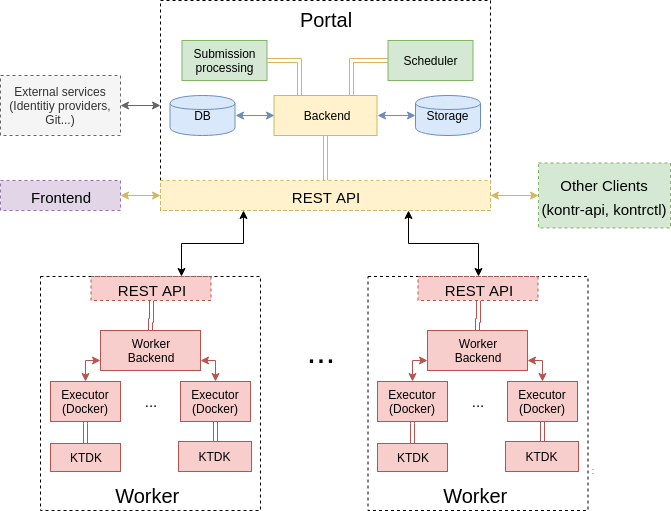
\includegraphics[width=\textwidth]{imgs/system-full.png}
  \end{center}
    \caption{Schéma systému Kontr 2}
    \label{fig:kontr2}
\end{figure}

\section{Portál}

Portál, hlavný komponent celého systému, bol navrhnutý a implementovaný v~bakalárskej práci Bc. Barbory Kompišovej\cite{kontr-portal}. Jeho hlavnou úlohou je vytvoriť \emph{logickú štruktúru entít} slúžiacich na modelovanie výukového procesu a vzťahov medzi nimi. Druhou úlohou Portálu je vystaviť \emph{rozhranie}, vďaka ktorému je možné systém ovládať a komunikovať s~ostatnými komponentmi v~systéme. Portál toto rozhranie zabezpečuje a implementuje \emph{mechanizmy riadenia prístupu}\cite{RFC4949}. Na uchovávanie stavu systému v~podobe jednotlivých entít a ich atribútov Portál využíva relačnú databázu, pretože tieto dáta sú štrukturované a je v~nich potrebné efektívne vyhľadávať.

Ako orchestrátor systému je Portál primárnym miestom spracovávajúcim hlavný prípad použitia -- vytvorenie odovzdania. Pre jedno odovzdanie ide v~následnosti o~tieto kroky: 

\begin{enumerate}
  \item prijať odovzdanie a jeho parametre od študenta
  \item skontrolovať potrebné oprávnenia a obmedzujúce podmienky na počet a frekvenciu odovzdaní
  \item stiahnuť a uložiť súbory potrebné pre spracovanie odovzdania, predovšetkým študentovo riešenie
  \item naplánovať vykonávanie odovzdania na Pracovníkovi a odoslať mu nové odovzdanie na spracovanie
  \item prijať výsledok spracovania od Pracovníka, uložiť a vyhodnotiť~ho
  \item notifikovať relevantných používateľov -- autora a opravujúceho tohoto odovzdania.
\end{enumerate}

Primárnou časťou Portálu je server, ktorý vystavuje \emph{REST rozhranie}\cite{fielding}, pomocou ktorého je možné s~Portálom komunikovať. Na rozhranie Portálu je možné napojiť rôznych klientov. Hlavnými výhodami REST rozhrania je jeho väzba na \emph{HTTP protokol}\cite{RFC2616} a možnosť zabezpečenia pomocou \emph{SSL/TLS protokolu}\cite{RFC8446}, umožňujúceho šifrovanie komunikácie. Podrobnejší popis rozhrania Portálu a rozpracovanie návrhových a implementačných otázok je možné nájsť v~spomínanej bakalárskej práci Bc. Barbory Kompišovej\cite{kontr-portal}.

\subsection{Klienti Portálu}
Vďaka jednotnému rozhraniu prispôsobenému pre automatizovanú prácu bolo pre Portál možné vyvinúť niekoľko samostatných klientov. 

\textbf{Frontend} pre systém Kontr 2 bol implementovaný ako súčasť práce Bc. Barbory Kompišovej\cite{kontr-portal}. Ide o~jednostránkovú webovú aplikáciu (\emph{single page application})\cite{single-page-app}, ktorá využíva REST rozhranie Portálu a ponúka možnosť spravovať entity v~systéme, vytvárať odovzdania a prezerať si výsledky. Rozšírením Frontendu bude nástroj na prezeranie odovzdaní (\emph{review tool}) sprístupňujúci rozhranie na prezeranie výsledkov a výstupov testovania, jednotlivých súborov odovzdania, pridávanie slovného hodnotenia vo forme komentárov k~súborom a prácu s~Poznámkovými blokmi IS~MU. 

Knižnica \textbf{kontr-api} implementovaná v~jazyku Python obaľuje volania REST rozhrania Portálu. Slúži ako základ pre písanie nástrojov v~jazyku Python, ktoré potrebujú pracovať a komunikovať so systémom Kontr 2. V~súčasnosti ju využívajú dva projekty: konzolový nástroj \emph{kontrctl (\fullref{impl-other-parts})}, pomocou ktorého je možné pracovať so serverovou častou Portálu a Pracovník, ktorý knižnicu používa na získanie informácii potrebných pre spracovanie odovzdania.


\subsection{Úložisko -- Storage}

Medzi interné nástroje obsiahnuté v~Portále patrí modul \emph{Úložisko (Storage)}, slúžiaci na ukladanie, spravovanie a spracovávanie súborov potrebných pri spracovaní odovzdania. Potenciálne ide o~veľké súbory, ktoré je potrebné členiť do stromovej štruktúry. Súbory je vhodné ukladať priamo na disk a využiť adresárovú štruktúru. Modul rozlišuje tri základné druhy súborov: 

\textbf{Študentovo riešenie} obsahuje predovšetkým zdrojové kódy, nad ktorými bude vykonávané testovanie. Je potrebné ukladať tieto súbory oddelene pre každé odovzdanie (napr. v~samostatných priečinkoch), aby bolo možné vždy k~odovzdaniu priradiť súbory, nad ktorými prebehlo testovanie.

\textbf{Testovacie súbory} označujú súbory potrebné na spustenie testov. Patria medzi ne súbory s~popisom testovacích scenárov (napr. jednotkové testy), vzorové vstupy, očakávané výstupy či čiastočné implementácie riešenia, umožňujúce izolované testovanie častí odovzdania. Tieto súbory je možné zdieľať pre spracovanie všetkých odovzdaní v~projekte, nemá zmysel ich kopírovať ku každému odovzdaniu.

\textbf{Výsledky testov} sú súbory vygenerované počas spracovania odovzdania. Ide predovšetkým o~výstupy spustených programov, napríklad záznam kompilácie a výstup testovacích rámcov. Je ich potrebné jednoznačne priradiť k~odovzdaniu.

Súčasťou Úložiska je integrácia s~Gitom, pomocou ktorého nástroj sťahuje odovzdania študentov a testovacie súbory. Pre úsporu miesta na disku modul ponúka možnosť filtrovania ukladaných dát pomocou \emph{glob výrazov\footurl{https://docs.python.org/3/library/glob.html}} (tzv. \emph{whitelist}) pri sťahovaní odovzdaní a kompresie priečinkov pri ich nevyužívaní.

\subsection{Asynchrónne spracovanie odovzdaní}
\label{design-async-process}

Pre webové aplikácie je jednou z~požiadaviek aj svižnosť -- po odoslaní požiadavky je odpoveď doručená v~krátkom časovom intervale. Protokol HTTP\cite{RFC2616} kvôli tomu obsahuje mechanizmus tzv. \emph{timeoutov}\footurl{https://developer.mozilla.org/en-US/docs/Web/HTTP/Status/408}. Rýchlu, neblokujúcu odpoveď je možné zabezpečiť \emph{asynchrónnym spracovaním úloh}, kedy je pri prijatí požiadavky vytvorená asynchrónna úloha, ktorá je spracovaná na pozadí. Odpoveďou na túto požiadavku môže byť napríklad informácia o~zaradení úlohy do frontu asynchrónnych úloh. Na samotný výsledok je potrebné vytvoriť samostatnú požiadavku.

Úlohy v~Portáli využívajúce asynchrónne spracovávanie:

\begin{itemize}
    \item Stiahnutie vypracovania odovzdania študenta
    \item Stiahnutie testovacích súborov
    \item Príprava prostredia pre odovzdanie
    \item Naplánovanie spracovania odovzdania na voľného Pracovníka
    \item Spracovanie výsledku testov odovzdania
\end{itemize}

Medzi štandardné možnosti asynchrónneho spracovania úloh je použitie metód paralelného spracovania pre daný jazyk, napríklad použitie vlákien alebo procesov. Využitie vlákien je v~mnohých interpretovaných jazykoch problematické, pretože implementácie ich interpretov nepodporujú súčasné spracovanie vlákien. Problémom je tzv. \emph{GIL - Global Interpreter Lock (Globálne uzamknutie interpretéra)} -- ide o~zámok, ktorý chráni natívne objekty v~jazyku a zabraňuje viacerým vláknam súbežné vykonávanie. Tento problém má aj \emph{CPython}, implementácia interpretéra jazyka Python, implementovaná v~jazyku C, na ktorej je celý projekt postavený\cite{cpython-gil}.

Druhou možnosťou je spustenie samostatných procesov, ktoré budú úlohy spracovávať. Najlepšou metódou je použiť už existujúce riešenie, ktoré odtieňuje od problémov distribuovaného spracovávania, ako je napríklad synchronizácia, plánovanie, výpadky a prenos dát pri distribuovanom spracovaní. Dostupné systémy sú založené na \emph{distribuovanom fronte úloh (distributed task queue)}, do ktorého \emph{producenti} vkladajú úlohy pripravené na spracovanie a \emph{konzumenti} úlohy z~frontu vyberajú postupne ich spracúvajú. Ide o~\emph{messaging} vzor \emph{publish-subscribe}\cite{ethomas-soa}.

Synchronizačný mechanizmus, ktorý v~sebe obsahuje front úloh sa volá tzv. \emph{sprostredkovateľ správ/úloh (Message Broker)}, ktorý zabezpečuje validáciu, verifikáciu, transformáciu a smerovanie správ správ medzi odosielateľom (producentom) a prijímateľom (konzumentom)\cite{mom}.

Producent, konzumenti aj sprostredkovateľ správ bežia ako samostatné procesy, ktoré je možné mať nasadené na separátnych strojoch, jediným prvkom dostupným producentom aj konzumentom musí byť len sprostredkovateľ. Producentom (\emph{publisher}) je REST rozhranie, ktoré sa v~kontexte webových aplikácii volá \emph{prijímač (listener)}, a konzumentom (\emph{subscriber}) je tzv. \emph{asynchrónny pracovník (asynchronous worker)}.

\begin{figure}[!ht]
  \begin{center}
    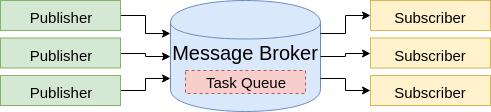
\includegraphics[width=\textwidth]{imgs/task-queue.png}
  \end{center}
    \caption{Schéma producent/konzument s~asynchrónnym frontom úloh}
    \label{fig:task-queue}
\end{figure}

\subsection{Plánovače}
\label{portal-scheduler}

Portál obsahuje dva typy plánovačov, ktoré ovládajú proces spracovania odovzdania. Ich úlohou je zabrániť preťažovaniu systému a~umožniť využívanie rôznych behových prostredí.

Prvý plánovač slúži na vypočítanie minimálneho časového rozostupu medzi odovzdaniami, tzn. kedy je študentovi povolené vytvoriť nové odovzdanie a a začať ho spracovávať. Konfigurácia plánovača je súčasťou projektu. Jednoduchým príkladom nastavenia plánovača je definovanie fixnej doby čakania. Ďalšou možnosťou je progresívne zvyšovanie minimálnej doby medzi odovzdaniami na základe celkového počtu odovzdaní študenta.

Druhý plánovač na základe definovaných kritérií rozhoduje, na ktorom Pracovníkovi bude vykonané odovzdanie. Do plánovacieho procesu vstupuje vyťaženie a dostupnosť Pracovníkov, prítomnosť služieb či nástrojov na jednotlivých Pracovníkoch a obmedzujúce podmienky definované správcom systému a zadávajúcim domácej úlohy. Príkladom obmedzení na Pracovníka je maximálna miera vyťaženia systémových prostriedkov, preferovaná platforma (operačný systém, jeho verzia) alebo obmedzenie, že daný Pracovník môže byť využívaný len určitou skupinou predmetov, projektov alebo študentov. 

Oba typy plánovačov sú súčasťou ešte nedokončenej bakalárskej práce \emph{Mateja Dujavy}\cite{kontr-scheduler}, ktorý sa v~svojej práci podrobne venuje návrhu a implementácii oboch plánovačov a ich integrácii so systémom Kontr~2.

\subsection{Nástroj na spracovanie odovzdania -- Submission processing}

Ďalším komponentom Portálu je \emph{Nástroj na spracovanie odovzdania (Submission processing)}. Skladá sa z~dvoch častí konfigurovateľných zadávajúcim úlohy. Prvou časťou je definícia akcií, ktoré sa majú vykonať pred odoslaním odovzdania na Pracovníka (tzv. \emph{preprocessing}). Medzi tieto úlohy patrí napríklad odoslanie emailu študentovi o~vytvorení nového odovzdania.

Druhou fázou je spracovanie výsledkov odoslaných z~Pracovníka do Portálu \emph{(postprocessing)}. Tu je možné definovať napríklad spracovanie výsledkov z~Pracovníka, nastavenie bodov a stavu odovzdania, odoslanie emailu autorovi a opravujúcemu či zápis bodov do Poznámkových blokov IS~MU na základe typu odovzdania. 

Spracovanie odovzdania a nastavenie vykonávaných úloh je prispôsobiteľné a modulárne. Každý predmet alebo zadávajúci si môže vybrať zo škály rôznych akcii, ktoré sa majú v~jednej z~častí vykonať.

Nástroj na spracovanie odovzdania je opäť súčasťou práce \emph{Mateja Dujavy}\cite{kontr-scheduler}, v~ktorej sa podrobne venuje návrhu a implementácii.

\subsection{Zdroje užívateľských identít a autentizácia}

Fakultná inštancia GitLabu je jedným zo systémov, s~ktorými Kontr 2 potrebuje komunikovať pre využitie metódy autentizácie používateľov \emph{OpenID Connect}\footnote{\url{https://openid.net/specs/openid-connect-core-1_0.html}}, kde GitLab pre Kontr 2 predstavuje \emph{poskytovateľa identít}. Pomocou napojenia na fakultnú \emph{LDAP databázu\footurl{https://tools.ietf.org/rfc/rfc4511.txt}} je možné od GitLabu získať údaje o~študentoch a učiteľoch na FI MU, čo umožňuje automatické vytváranie dôveryhodných používateľských účtov. Pre administráciu systému, umožnenie prístupu osobám neregistrovaným vo fakultnej databáze účtov a vnútornú organizáciu systému je však v~Portáli stále nutné implementovať vlastnú správu účtov. 

Na získanie dodatočných informácii o~užívateľovi je potrebné Portál integrovať aj s~fakultnou LDAP databázou, ktorá je dostupná len zo siete FI MU. Jednou z~dôležitých informácii, ktoré odtiaľto Portál získava je UČO (univerzitné číslo osoby) užívateľa. To je uložené v~atribúte \emph{description} v~LDAP zázname každého užívateľa.

\subsection{Email}
Pre možnosť odosielania emailových správ užívateľom je potrebné Portál integrovať s~SMTP serverom\footurl{http://www.rfc-editor.org/rfc/rfc5321.txt}. Obsah správ a podmienky ich odosielania je možné upraviť na úrovni Kontr~2. Správy systém generuje automaticky na základe definovaných šablón a dodaných parametrov. Adresátov je možné filtrovať na základe ich členstva v~kurze, skupine a ich rolí. Podnetom na odoslanie emailovej správy môžu byť napríklad tieto udalosti: vytvorenie užívateľa, zmena užívateľovho hesla, zmena členstva užívateľa v~skupine alebo zmena jeho roly v~danom predmete.

\subsection{Poznámkové bloky IS MU}
Okrem emailových správ systém používateľom poskytuje spätnú väzbu aj pomocou Poznámkových blokov IS MU. Poznámkové bloky typicky obsahujú bodové, prípadne slovné hodnotenie študentských výsledkov. V~prípade Kontru 2 ide o~zápis redukovaného výsledku automatických testov. Na základe konfigurácie je možné automaticky zapisovať hodnotenie záväzne, prípadne vyžadovať manuálne potvrdenie výsledkov. Práca s~rozhraním Poznámkových blokov IS MU vyžaduje prístupový token, ktorý môžu vyučujúci generovať v~IS MU.

Implementácia tejto služby nie je súčasťou tejto práce, no je dôležitá pre reálne využitie systému Kontr 2 v~ostrej prevádzke.

\subsection{Knižnica na správu a komunikáciu s~Pracovníkom}
Súčasťou Portálu je aj knižnica na komunikáciu s~Pracovníkom a jeho správu. Pomocou nej je možné zistiť stav aktuálne vykonávaného odovzdania, spustiť spracovanie odovzdaného riešenia alebo zistiť jeho aktuálne vyťaženie či zoznam definovaných štítkov.

\section{Pracovník}
Pojem \emph{Pracovník (Worker)} v~systéme Kontr 2 naberá význam na dvoch úrovniach. Ako koncept označuje nástroj, ktorého vstupom je odovzdanie spolu s~popisom testovacích scenárov a výstupom je sada definovaných súborov, potrebných pre spracovanie a vyhodnotenie výsledkov testovania. Ako jeden z~hlavných komponentov systému predstavuje konkrétnu implementáciu spomínaného konceptu -- samostatnú jednotku, ktorej účelom je vykonávať odovzdania na určitom stroji a platforme. 

Koncept Pracovníka je možné implementovať rôznymi spôsobmi, ktoré sú prispôsobené danému prípadu použitia. Konkrétne implementácie odrážajú potreby predmetov využívajúcich systém Kontr 2 -- požadované platformy, výhody, služby a zdroje definovaného behového prostredia. Každá implementácia Pracovníka musí spĺňať určité požiadavky, predovšetkým musí vystaviť definované REST rozhranie na umožnenie komunikácie s~Portálom. 

Konkrétna implementácia Pracovníka je jedným z~výstupov tejto práce a bola použitá pri testovacej prevádzke. Ide o~Pracovníka implementovaného pre platformu Linux využívajúceho \emph{kontajnerizačnú technológiu}\footnote{\url{https://opensource.com/resources/what-are-linux-containers}}. Využitie kontajnerov v~Pracovníkovi umožňuje lepšiu izoláciu a riadenie práv spúšťaných testovacích procesov. Táto implementácia je zamýšľaná ako vzor pre ďalšie špecifické riešenia. Pre využitie platformy \emph{MS Windows}\footurl{https://www.microsoft.com/en-us/windows} bude potrebné overiť možnosť využitia spomínanej kontajnerizačnej technológie a prípadne vyhodnotiť dostupné alternatívy.

\subsection{Priebeh spracovania}

Prijatie a spracovanie odovzdania Pracovníkom prebieha v~troch fázach:

\begin{enumerate}
    \item Príprava prostredia, počas ktorej sú získané všetky potrebné dáta a informácie potrebné pre spracovanie odovzdania
    \item Spustenie testovacích scenárov nad odovzdaním a vygenerovanie výsledkov
    \item Spracovanie výsledkov do očakávanej výstupnej podoby a ich odoslanie do Portálu
\end{enumerate}

Portál odošle Pracovníkovi správu o~vytvorení nového odovzdania, ktoré je potrebné spracovať. Pracovník overí, či správa pochádza od jemu známej inštancie Portálu a zodpovedá jeho možnostiam.  V~prípade, že overenie zlyhá, požiadavka je zamietnutá. Zo správnej požiadavky extrahuje základné informácie o~odovzdaní -- identifikáciu odovzdania, autora, projektu, pre ktorý bolo odovzdanie vytvorené a dodatočné parametre potrebné pre jeho vykonanie. Následne Pracovník od Portálu vyžiada súbory obsahujúce riešenie študenta a súbory potrebné na spustenie testovacích scenárov. Získané dáta sú uložené a pripravené na spracovanie. 

Priebeh ďalšieho spracovania je závislý na konkrétnej implementácii Pracovníka. Je pritom potrebné zabezpečiť, aby spracovávané súbory a programy nekompromitovali systém Pracovníka (nespôsobili jeho pád alebo poškodenie, nesprístupnili citlivé dáta neoprávneným používateľom, nemanipulovali s~priebehom vyhodnotenia). 

Po vykonaní testovacích scenárov Pracovník odošle ich výsledky Portálu na spracovanie. Výsledky musia spĺňať formát definovaný v~Portále (\emph{postprocess konfigurácia nástroja na spracovanie odovzdania} pre projekt), aby ich bolo možné správne interpretovať a vyhodnotiť. Pre tento účel Portál vystavuje v~rozhraní špeciálny koncový bod. Odoslaním výsledku spracovania Portálu končí spracovanie odovzdania v~Pracovníkovi.

\subsection{Návrh Pracovníka s~využitím linuxových kontajnerov}
\label{design-worker-lc}

Na demonštračné účely v~rámci testovacieho nasadenia Kontru 2 bolo potrebné detailne rozpracovať a implementovať koncept Pracovníka. Dodaná implementácia má podobnú štruktúru ako Portál: vystavuje REST rozhranie v~časti nazvanej \emph{prijímač} a spracovanie dlhotrvajúcich úloh zabezpečujú asynchrónni pracovníci. Prostredníka medzi prijímačom a asynchrónnym pracovníkom zabezpečuje \emph{message broker}. Komplexnejšie predstavenie celej architektúry s~dôvodmi a výhodami využitia týchto princípov sú popísané v~časti \fullref{design-async-process}. 

Spracovanie jednotlivých odovzdaní je zabezpečené pomocou \emph{kontajnerizačnej technológie}, vďaka ktorej je možné spúšťať testovacie scenáre v~bezpečnejšom a odtienenom prostredí. Kontajnerizačná technológia je založená na metóde virtualizácie na úrovni operačného systému, ktorá umožňuje beh viacerých izolovaných linuxových systémov na jednom zdieľanom jadre operačného systému\cite{linux-containers-rh}. 

Jednou z~najznámejších kontajnerových platforiem je produkt \emph{Docker}\footnote{\url{https://www.docker.com/}}, ktorý implementácia využíva. Základnými jednotkami v~platforme Docker je tzv. \emph{obraz (image)}, na základe ktorého je možné spúšťať mnoho \emph{kontajnerov} -- inštancií daného obrazu. Kontajnery izolujú spúšťané služby od hostiteľského systému a zaručujú tak ľahkú prenositeľnosť medzi rôznymi behovými prostrediami (servermi)\cite{docker-stuff}. Alternatívou k~produktu Docker sú napríklad \emph{rkt}\footurl{https://coreos.com/rkt/} od firmy Core OS (odkúpenej firmou Red Hat) alebo \emph{LXD}\footurl{https://linuxcontainers.org/lxd/introduction/} od firmy Canonical. 

Všetky odovzdania sú vykonávané izolovane a je ich možné oddeliť od určitých zdrojov fyzického stroja, napríklad siete, pomocou ktorej by mohol sprístupniť citlivé informácie. Rovnako v~prípade chyby alebo spustenia nevhodných alebo nebezpečných programov dôjde len k~poškodeniu alebo kompromitovaniu (ľahko nahraditeľného) kontajnera, nie celého systému. Ďalšou výhodou je možnosť prispôsobenia testovacieho prostredia: do obrazu je možné vložiť konkrétne verzie potrebných nástrojov (prekladač, valgrind apod.) bez ohľadu na hosťovský systém.

Základom kontajnerov používaných na testovanie odovzdaní v~Pracovníkovi sú obrazy obsahujúce všetky potrebné nástroje. Inštrukcie potrebné na jeho zostavenie sú súčasťou definície testovacích scenárov. Pracovník si testovacie obrazy rôznych úloh rôznych predmetov uchováva v~\emph{lokálnom registre obrazov}\footnote{\url{https://docs.docker.com/registry/}} dovtedy, kým nedôjde k~zmene testovacích súborov. Vďaka tomu je proces testovania rýchlejší -- obrazy nie je potrebné zostavovať pre každé odovzdanie zvlášť. Obrazy sú pripravené pred spustením odovzdávania a spravované centrálne.

Spracovanie každého odovzdania je spúšťané v~samostatnom kontajneri, ktorý z~bezpečnostných dôvodov nemá prístup k~sieti. Študentovo vypracovanie je do kontajneru vložené pomocou \emph{perzistentného zväzku (persistent volume)}\footnote{https://docs.docker.com/storage/volumes/}, ktoré kontajner smie len čítať \emph{(read-only)}, vďaka čomu nie je možné odovzdanie počas testov modifikovať. Do kontajneru je podobne vložený aj priečinok, do ktorého spracovanie zapíše výsledky testovania. Tento priečinok je po skončení spracovania zabalený a odoslaný Portálu.

\subsection{Rozhranie}

Pracovník môže byť implementovaný rôznymi spôsobmi, samotné spracovanie odovzdania je závislé na potrebách a obmedzeniach daného predmetu alebo úlohy. Každá implementácia Pracovníka ale musí vedieť korektne odpovedať na nasledujúce požiadavky, ktoré sú nevyhnutné pre správny chod Portálu:

\begin{itemize}
    \item Registrácia Pracovníka do Portálu
    \item Požiadavka na aktuálny stav Pracovníka
    \item Požiadavka na začatie spracovania odovzdania
    \item Požiadavka ukončenie spracovania odovzdania
    \item Požiadavka na aktuálny stav odovzdania
\end{itemize}

\textbf{Registrácia Pracovníka do Portálu} je nevyhnutná na ustanovenie zabezpečeného spojenia medzi Portálom a Pracovníkom. Bližší popis sa nachádza v~časti \fullref{komunikacia-portal-pracovnik}.

\textbf{Požiadavka na aktuálny stav} informuje Portál o~aktuálnom vyťažení Pracovníka, potrebnom pre plánovač Portálu. Odpoveď na tento dotaz musí obsahovať informácie o~maximálnom počte paralelných spracovaní odovzdaní, ktoré je Pracovník schopný spracovať a aktuálny počet spracovávaných odovzdaní. Odpoveď môže obsahovať dodatočné informácie, napríklad vyťaženie prostriedkov stroja \emph{(load)}.

\textbf{Požiadavka na spracovanie odovzdania} obsahuje identifikátor odovzdania, informáciu o~projekte, kurze, autorovi odovzdania a dodatočné parametre, ktoré sú potrebné pre beh testov, napríklad parametre pre testovací rámec \emph{KTDK}. Požiadavka je odoslaná Portálom po tom, čo je odovzdanie pripravené, tzn. všetky potrebné súbory boli stiahnuté a uplynula nastavená minimálna doba čakania.

\textbf{Požiadavka na aktuálny stav odovzdania} informuje Portál o~aktuálnom stave spracovania odovzdania s~cieľom zistiť prípadné chyby pri spracovaní. Odpoveď by okrem stavu mala obsahovať aj dodatočné informácie, ktoré môžu pomôcť pri hľadaní a oprave chyby.

\emph{Požiadavka na ukončenie spracovávania odovzdania} je potrebná ak došlo k~chybe spracovania a je ho potrebné násilne ukončiť.

\section{Komunikácia medzi Portálom a Pracovníkom}

Komunikácia medzi Portálom a Pracovníkom prebieha pomocou REST rozhraní na strane Pracovníka a Portálu. 

\subsection{Vzájomná autentizácia}
\label{komunikacia-portal-pracovnik}

Rozhranie Portálu aj Pracovníka je zabezpečené pomocou autentizačného tokenu. Pracovník si generuje vlastný autentizačný token, ktorý používa Portál na autentizáciu požiadaviek smerovaných na Pracovníka. Pracovník na autentizáciu požiadaviek na Portál používa \emph{prístupový token}, ktorý mu vygeneroval Portál na základe prihlásenia pomocou tajomstva Pracovníka.

Registrácia novej inštancie Pracovníka je znázornená v~diagrame \ref{fig:worker-reg}. Proces začína vytvorením entity Worker s~parametrami \emph{URL Pracovníka}, \emph{meno Pracovníka} v~Portáli a nastavením jeho tajomstva (\emph{secret}). Po štarte Pracovníka sa pomocou tohoto tajomstva a svojho mena Pracovník autentizuje voči Portálu na známej URL, čím získa prístupový token. Následne Portálu pošle svoj (nový) token, ktorý Portál uloží a pripája ku všetkým nasledujúcim dotazom na Pracovníka. Tento token slúži na autentizáciu Portálu voči Pracovníkovi. Neprítomnosť alebo nerozpoznanie tohoto tokenu v~požiadavke znamená jej zamietnutie Pracovníkom. Po úspešnej registrácii je Pracovník pripravený spracovávať odovzdania.

Súčasťou registrácie Pracovníka je aj zaregistrovanie \emph{štítkov (feature tags)} v~Portáli, ktoré následne využíva plánovač Portálu pre rozdeľovanie odovzdaní medzi rôznych Pracovníkov. Štítky informujú o~možnostiach a dostupných funkciách daného Pracovníka, napríklad aký operačný systém je na Pracovníkovi nainštalovaný či akú kontajnerizačnú technológiu daný Pracovník podporuje. 

\begin{figure}[!ht]
  \begin{center}
    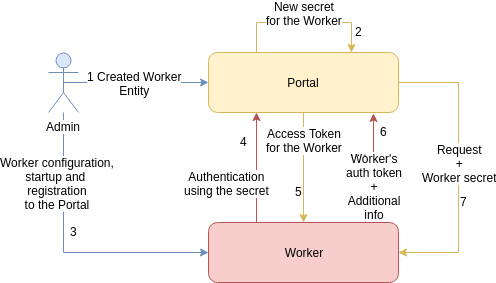
\includegraphics[width=\textwidth]{imgs/worker-reg.png}
  \end{center}
    \caption{Schéma procesu registrácie Pracovníka do Portálu}
    \label{fig:worker-reg}
\end{figure}

\subsection{Spracovanie odovzdania}
Portál pri výbere vhodného Pracovníka na spracovanie nového odovzdania zohľadňuje aktuálny stav Pracovníka, ktorý získa pomocou požiadavky na stav. O~samotný výber sa stará plánovač, popísaný v~časti \fullref{portal-scheduler}. Vybranému Pracovníkovi sa odosiela požiadavka na spracovanie odovzdania. Po jej skontrolovaní a prijatí Pracovník od Portálu vyžiada potrebné súbory. Po skončení spracovania odovzdania Pracovník nahrá riešenie do Úložiska Portálu, čím aktualizuje stav a výsledok odovzdania v~Portáli. Ak výsledky nedorazia v~definovanom čase, Portál od Pracovníka zisťuje stav odovzdania. V~prípade, že je detekovaná chyba, Portál odošle požiadavku na zastavenie vykonávania a pokúsi sa spustiť spracovanie odovzdania znova. 

\section{Testovací rámec KTDK - Kontr test development kit}

\emph{KTDK -- Kontr test development kit} je testovací rámec slúžiaci na popis scenárov, pomocou ktorých je možné testovať a vyhodnotiť odovzdania študentov.

Rámec je samostatný komponent a používa sa ako knižnica, ktorá je voľne dostupná\footnote{\url{https://pypi.org/project/ktdk/}}. Testy definované pomocou rámca \emph{KTDK} sú Python skripty, ktoré sú majú väzbu na konkrétnu verziu rámca, čím je zabezpečená spätná kompatibilita. Nástroj je nezávislý od ostatných komponent systému Kontr~2, čo umožňuje využívať lokálnu inštaláciu rámca  otestovanie funkčnosti alebo ladenie testov s~dodaným riešením. Spúšťanie testovacích scenárov prebieha spustením skriptu s~ich definíciou v~pripravenom prostredí.

Pre definíciu testovacích scenárov bolo potrebné navrhnúť štruktúru a model vykonávania testov, ktorý bude ľahko rozšíriteľný a modifikovateľný. Rozhodnutie implementovať vlastný testovací rámec vyplynulo zo špecifických požiadaviek jednotlivých predmetov, predovšetkým ich rôznych postupov a nástrojov, ktoré sa pri testovaní využívajú. V~niektorých predmetoch sa využívajú testy definované v~existujúcom testovacom rámci pre daný jazyk (\emph{JUnit, Catch2, pytest}), iné využívajú porovnávanie výstupov aplikácie s~očakávanými, pripravenými výstupmi. Ďalej bolo potrebné umožniť kontrolu riešení pomocou externých nástrojov, napr. \emph{Valgrind, Checkstyle, Clang-tidy, Clang-format, a ďalšie}.

Na rozdiel od štandardných testovacích nástrojov KTDK oddeľuje definíciu testovacích scenárov od výkonného kódu testov aj testovaného kódu. \emph{Testované súbory} obsahujú zdrojové kódy odovzdané študentom a \emph{testovacie súbory} sú súbory obsahujúce výkonný kód testov, spúšťaný pomocou KTDK. K~testovacím súborom je možné zaradiť aj rôzne podporné časti potrebné na testovanie študentovho odovzdania -- pripravené vstupy, čiastočné implementácie apod.

Testovanie pomocou KTDK je možné na konceptuálnej úrovni rozdeliť do niekoľkých fáz:
\begin{enumerate}
    \item \emph{Príprava prostredia}: skombinovanie dodaných testovacích a testovaných súborov.
    \item \emph{Kompilácia}: preloženie dodaných súborov do binárnej podoby.
    \item \emph{Spustenie testov nad binárnymi súbormi}: spustenie jednotlivých testov nad výstupom kompilácie
    \item \emph{Spracovanie výsledkov testovania} -- vyhodnotenie výsledkov a výstupov spracovania nástrojmi a priradenie výsledku príp. bodov pre jednotlivé testy
    \item \emph{Vytvorenie výstupu} -- celkový výstup, ktorý je možné spracovať v~Portáli a ohodnotiť pomocou neho študentovo odovzdanie.
\end{enumerate}

Rôzne technológie a jazyky ale vyžadujú rozdielny priebeh testovania (napr. pre interpretované jazyky nie je potrebná kompilácia), preto je uvedený zoznam skôr orientačný. Scenáre sú v~KTDK modulárne, ich výsledná podoba preto môže byť pre potreby každého predmetu a úlohy iná. 

\subsection{Štruktúra priečinkov}

\begin{figure}[!ht]
  \begin{center}
    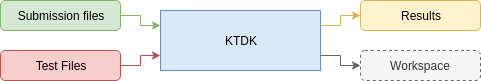
\includegraphics[width=\textwidth]{imgs/ktdk-io.png}
  \end{center}
    \caption{Vstupy a výstupy pre KTDK}
    \label{fig:ktdk-io}
\end{figure}

Rámec na vstupe očakáva cesty k~štyrom priečinkom (obr. \ref{fig:ktdk-io}):
\begin{itemize}
    \item \emph{Priečinok s~vypracovaním (testované súbory)} obsahujúci pripravené odovzdanie študenta, ktoré bude testované.
    \item \emph{Priečinok s~testovacím súbormi} obsahujúci testovacie scenáre a súbory potrebné na testovanie.
    \item \emph{Priečinok s~výsledkami}, do ktorého budú uložené výsledky testovania.
    \item \emph{Pracovný priečinok (workspace)}, do ktorého skopírujú súbory na základe definovaných pravidiel a v~ktorom sa bude vykonávať samotné spustenie testov. Pracovný priečinok je po skončení testov zahodený, pretože môže obsahovať výstupy, ktoré nie sú potrebné (napríklad vygenerované binárne súbory).
\end{itemize}

\subsection{Logická štruktúra testovacích scenárov}
\label{design-struct-test-scenarios}
KTDK definuje dva hlavné štrukturálne komponenty: \emph{test} a \emph{úlohu (task)}. Test je definovaný svojím \emph{menom, popisom, bodovým ohodnotením a štítkami (\emph{tags})} a tvorí "obálku" pre určitú časť testovacieho scenára. Testy je možné do seba zanorovať a vytvoriť tak stromovú štruktúru, ktorá logicky člení scenár na lepšie spravovateľné časti a zároveň zoskupuje príbuzné či previazané testy. 

Na test je možné naviazať \emph{úlohy (task)}, predstavujúce konkrétne akcie s výkonným kódom, ktorý sa má počas testu vykonať. Rámec dodáva škálu základných akcií (napr. presúvanie súborov, kompilácia testov, spracovanie výstupu testovacích nástrojov) a umožňuje definíciu vlastných. Na test sa tiež viaže bodové hodnotenie a celkový výsledok, ktoré sú spočítané po skončení vykonávania testov. Podobne ako testy je možné zanorovať do seba aj úlohy a modelovať tak závislosti medzi nimi.

Každý test obsahuje päť kolekcií úloh, vykonávaných sekvenčne:
\begin{enumerate}
    \item Úlohy vykonané pred testom samotným \emph{(before all)}.
    \item Úlohy viazané na test \emph{(test's tasks)}
    \item Úlohy vykonané pred každým potomkom testu \emph{(before each)} 
    \item Úlohy vykonané po každom potomkovi testu \emph{(after each)}
    \item Úlohy vykonané po teste samotnom \emph{(after all)}.
\end{enumerate}

Existujú tri hlavné kategórie úloh:
\begin{itemize}
    \item \emph{Vykonávacie}, ktoré vykonávajú akcie a spracovávajú výsledky
    \item \emph{Kontrolované (checked)} slúžiace na overenie podmienok pre splnenie požiadaviek pre daný test a explicitné rozhodnutie o~výsledku jedného testu -- \emph{splnenie (\texttt{PASS})} alebo \emph{zlyhanie (\texttt{FAIL})}.
    \item \emph{Kontrolované vyžadované (required)} sa správajú rovnako ako kontrolované, ale v~prípade zlyhania kontroly dôjde k~ukončeniu aktuálne vykonávaného testu a všetkých jeho potomkov.
\end{itemize}

Pre úlohu je možné definovať meno, popis, informatívne štítky a koeficient redukovania počtu bodov za test. \emph{Redukčný koeficient} slúži sa zníženie počtu získaných bodov v~prípade, že úloha zlyhala a je \emph{kontrolovaná}. Východzia hodnota je nastavená na $0$: v~prípade zlyhania jednej úlohy sa predpokladá zlyhanie celého testu a výsledný priradený počet bodov za neúspešný test je nula. Pre testovanie výsledku nástrojom \emph{valgrind} je ale vhodné mať možnosť prideliť percentuálnu časť celkového počtu bodov, napr. s~koeficientom $0.7$ prideliť zlyhanej valgrind úlohe $70\%$ plného počtu bodov.

\subsection{Testovacie scenáre}

Testovanie scenáre je potrebné definovať pomocou \emph{KTDK} a dodaných entít. Testovací rámec je dodávaný ako knižnica jazyka \emph{Python} a preto sa aj scenáre definujú pomocou neho. Vďaka tomu je možné testovací rámec ľahko rozšíriť o~potrebnú funkcionalitu alebo upraviť podľa vlastných predstáv. 

Spustenie spracovania testovacích scenárov je rozdelené do troch fáz:
\begin{enumerate}
    \item \emph{Načítanie testovacieho scenára}, pri ktorom dôjde k~spracovaniu scenára a vybudovaniu stromu závislostí (testov a priradených úloh). Načítanie a budovanie stromu je zabezpečené pomocou konceptov a štruktúr (objektová hierarchia, kolekcie) v~jazyku Python.
    \item \emph{Spustenie testovacieho scenára}, pri ktorom dôjde k~vykonaniu definovaných úloh v~strome a uloženia výsledkov pre dané testy a úlohy.
    \item \emph{Spracovanie výsledkov}, počas ktorého sú spracované a vyhodnotené čiastkové výsledky do jednotného výsledku a výstupu celého testovania.
\end{enumerate}

\subsection{Spustenie testovacieho scenára}

Spustenie testovacieho scenára je vykonávané pomocou jednotky nazvanej \emph{spúšťač (runner)}. Spúšťač je definovaný pre každý \emph{test} a \emph{úlohu}. Jeho hlavnými úlohami sú vloženie \emph{kontextu (context)} do bezstavového testu alebo úlohy a určenie poradia vykonávania úloh a potomkov testov. 

\subsection{Kontext}

\emph{Kontext} je entita reprezentujúca postupne predávaný stav medzi úlohami a testami. Slúži ako jediné možné úložisko premenných a konfigurácie, ktoré je potrebné medzi testami a úlohami zdieľať. Jednotlivé časti kontextu sa postupne kopírujú po jednotlivých vetvách stromu zhora nadol. Príkladom využitia kontextu je úloha na kompiláciu, ktorá do kontextu uloží cesty k~vytvoreným súborom a nasledujúca úloha spustí testy nad práve týmito súbormi.


Kontext je vkladaný do testov a úloh až spúšťačom, preto nie je dostupný pri samotnej definícii testov, ale až vo fáze vykonávania testovacieho scenára.

Kontext má tri zložky:
\begin{itemize}
    \item \emph{Globálnu}, ktorá je definovaná globálnou konfiguráciou, predanou pri spustení celého scenára. Jej obsahom sú napríklad cesty k~jednotlivým priečinkom, globálne časové limity alebo prednastavené prepínače pre jednotlivé nástroje. 
    \item \emph{Testovú}, ktorá je viazaná na jeden test a je zdieľaná všetkými jeho potomkami a úlohami. Do testového kontextu môžu zapisovať len úlohy priamo naviazané na daný test. Pre každého potomka je tento kontext prístupný len na čítanie a úlohy potomkov k~nemu prístup nemajú.
    \item \emph{Kontext úlohy}, ktorý je viazaný len na aktuálnu úlohu, ktorá do neho môže zapisovať a všetky jej podúlohy, ktoré ho môžu čítať.
\end{itemize}

Pre zjednodušenie práce sú všetky tri zložky pri čítaní zlúčené do jednej s~nasledujúcimi prioritami: najskôr sa prehľadáva kontext úlohy, následne kontext testu a ako posledný sa prehľadáva globálny kontext. Pri zápise premennej do kontextu je potrebné určiť, do ktorej jeho zložky sa má zapisovať. 

\subsection{Výber testu pre spracovanie}

Jednou z~úloh spúšťača je vybrať na základe definovaných kritérií testy, ktoré v~danom behu majú byť spustené. Hlavným rozhodovacím kritériom je vyhodnotenie \emph{štítkov testov (tags)}, jednoslovných označení, pomocou ktorých je možné testy filtrovať.

Metóda štítkov je založená na vyhodnocovaní \emph{logických výrazov} podľa štítkov prítomných na danom teste. Výraz obsahuje mená štítkov a na jeho vyhodnotenie sa využíva jazyk Python. Príkladom výrazu môže byť: \texttt{naostro and not štýly}, na základe ktorého sa vykonajú len tie testy, ktoré sú označené štítkom \texttt{naostro} a zároveň nie sú označené štítkom \texttt{štýly}. 

Pre vyhodnocovanie výrazov platia nasledujúce pravidlá:
\begin{itemize}
    \item Ak je výraz prázdny, vykonajú sa všetky testy bez obmedzení.
    \item Ak je výraz len jedno slovo, vykonajú sa všetky testy označené týmto slovom, ostatné sú preskočené.
    \item Ak je výraz negácia (\texttt{not <štítok>}), vykonajú sa všetky testy, ktoré nie sú označené týmto štítkom.
    \item Výraz môže byť zložený pomocou logických spojok: \texttt{and} a \texttt{or} v~obvyklom logickom význame.
    \item Výraz môže obsahovať zátvorky, vďaka ktorým je možné explicitne definovať prioritu vyhodnotenia. 
\end{itemize}

Vzhľadom na stromovú štruktúru testov je potrebné poskytnúť metódy propagácie štítkov:
\begin{enumerate}
    \item Potomkovia obsahujú všetky štítky definované priamo na ich rodičoch (propagácia smerom nadol)
    \item Rodičia obsahujú všetky štítky svojich potomkov (propagácia smerom nahor). Tieto štítky sa nešíria naspäť nadol.
\end{enumerate}

Príklad: Majme tri testy, A, B, a C, pričom A~je rodič testu B aj testu C (testy B a C sú súrodenci). Každý z~týchto testov má na seba naviazaný práve jeden štítok: A~obsahuje štítok $a$, B má $b$, C má $c$. 

Propagácia štítkov smerom nadol zaručí, že testy B a C budú obsahovať aj štítok $a$ tzn. všetky štítky ich predka. Vďaka tejto vlastnosti je zabezpečené, že ak sa majú spustiť všetky testy so štítkom $a$, tak sa spustí test označený týmto štítkom a všetci jeho potomkovia.

Propagácia štítkov smerom nahor spôsobí, že test A~bude efektívne obsahovať štítky $a$, $b$ a $c$. Potom v~prípade obmedzenia na spúšťanie '$b$' sa spustí test B a všetci jeho predkovia (test A). Dôvodom pre túto propagáciu je to, že predkovia testu B obsahujú akcie, ktoré je potrebné vykonať pred vykonaním B a po skončení jeho spracovania.

Po propagácii štítkov nahor sa štítky už nepropagujú naspäť nadol, tzn. B neobsahuje štítok $c$ a C neobsahuje štítok $b$. Inak povedané, dopočítané efektívne štítky sa nepropagujú.

Výsledné efektívne ohodnotenie štítkami pre tento príklad vyzerá nasledovne:
\begin{table}[h]
\begin{tabular}{c c c}
Test & Dodané štítky & Vyhodnotené efektívne štítky  \\ [0.5ex] 
\hline
A~& $\set{a}$ & $\set{a,b,c}$ \\
B & $\set{b}$ & $\set{a,b}$   \\
C & $\set{c}$ & $\set{a,c}$   \\
\end{tabular}
\end{table}


\subsection{Výsledky testov a úloh}

Výsledky testov a úloh môžeme rozdeliť na \emph{aktuálny výsledok}, ktorý nie je závislý na výsledkoch potomkov testu či úlohy a na \emph{efektívny výsledok}, ktorý zohľadňuje aj výsledky potomkov. V~prípade, že jeden z~potomkov zlyhal, je efektívny výsledok zlyhanie.

Rozlišujeme päť možných stavov pre výsledok:
\begin{itemize}
    \item Žiaden výsledok (\emph{none}) -- test alebo úloha ešte neprebehli.
    \item Úspešný výsledok (\emph{passed}) -- test alebo úloha uspeli.
    \item Preskočený výsledok (\emph{skipped}) -- test, všetky jeho úlohy a potomkovia boli preskočení.
    \item Zlyhaný výsledok (\emph{failed}) -- test alebo kontrola neprešli.
    \item Chyba v~teste (\emph{error}) -- test alebo úloha skončili s~chybou. Ide o~chybný test, chybu v~testovacom rámci alebo chybu prostredia.
\end{itemize}

\subsection{Proces spracovania testu}
\label{design-runner}

Pri spracovaní testu dochádza najskôr k~vytvoreniu jeho spúšťača, súčasťou ktorého je vytvorenie kontextu pre daný test. Táto časť popisuje spúšťač dodaný v~tejto práci, je ale možné implementovať vlastný spúšťač s~iným poradím akcii. 

Po vytvorení kontextu je podľa štítkov testu vyhodnotený dodaný logický výraz. V~prípade, že test zadanú podmienku nespĺňa, je jeho výsledok je nastavený na stav \emph{skipped} a pokračuje sa ďalším testom. V~opačnom prípade sa spustia \emph{before all} úlohy tohoto testu, následne všetky \emph{before each} úlohy z~rodičovského testu. Po nich nasledujú úlohy testu samotného. Ak všetky úlohy prebehnú v~poriadku a nedôjde k~ukončeniu vykonávania testu, rovnakým spôsobom sú vyhodnotené všetky dcérske testy. Po skončení spracovania potomkov sa spracovávajú \emph{after each} úlohy rodiča a \emph{after all} úlohy testu.

Pri spracovaní každej úlohy dôjde k~vytvoreniu \emph{spúšťača úlohy}, ktorý prechádza strom úloh, ktoré postupne spúšťa a priraďuje im výsledky. Súčasťou spracovania behu úlohy je kontrola správnosti jej vykonávania a vhodné reagovanie na prípadné chyby.

\subsection{Spracovanie výsledkov}

Fáza spracovania výsledkov nasleduje po skončení behu testovacích scenárov, dochádza k priechodu vybudovaného stromu testov a úloh s~pridelenými výsledkami, na základe ktorých je vypočítané výsledné bodové hodnotenie a extrahované informácie o~úspešných a neúspešných testoch.

Výstup fázy spracovania obsahuje: finálny výsledok, počet získaných bodov zaokrúhlený na štyri desatinné miesta, zoznam zlyhaných testov a úloh a zoznam všetkých definovaných testov s~výsledkami.

Výstup je uložený do priečinka s~výsledkami spolu s~výstupmi ostatných nástrojov, logom behu testov a zoznamom súborov vygenerovaných počas behu. Tento priečinok je predaný na spracovanie Pracovníkovi, ktorý jeho obsah odosiela Portálu.

\section{Celkový priebeh spracovania nového odovzdania}

\begin{figure}[h]
  \begin{center}
    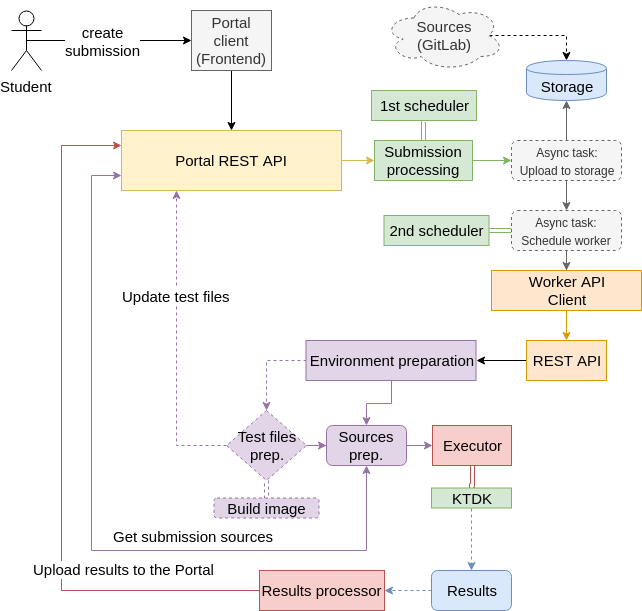
\includegraphics[width=\textwidth]{imgs/create-subm.png}
  \end{center}
    \caption{Diagram spracovania nového odovzdania}
    \label{fig:create-subm}
\end{figure}


Nové odovzdanie vytvorené študentom je odoslané na rozhranie Portálu (obr. \ref{fig:create-subm}). Pri vytvorení nového odovzdania dochádza ku kontrole oprávnení užívateľa a obmedzení kladených na zamedzenie zneužívania systému alebo prekročeniu definovaných limitov. V~prípade nesplnenia vyžadovaných kritérií je nové odovzdanie zamietnuté. Kontrola obmedzení prebieha v~prvom plánovači Portálu, ktorý zohľadňuje definované pravidlá pre danú úlohu (napríklad študent smie odovzdať vypracovanie len za určitý časový interval).

V~prípade, že odovzdanie je povolené, uložia sa všetky potrebné informácie o~odovzdaní a dáta potrebné na jeho spracovanie a vyhodnotenie. Pre odovzdanie je nastavený časový interval, počas ktorého je možné odovzdanie zrušiť.

Po uplynutí časového intervalu je spracovanie presunuté do fázy prípravy, v~ktorej dôjde k~stiahnutiu potrebných súborov a ich uloženie na \emph{Úložisko}.

Následne sa v~druhom plánovači vyberie najvhodnejší Pracovník pre spracovanie odovzdania. V~prípade, že žiaden Pracovník nie je dostupný je spracovanie odovzdania odložené na neskôr.

Po úspešnom výbere Pracovníka nasleduje jeho notifikácia o~novom odovzdaní. Po prijatí notifikácie Pracovník stiahne súbory prináležiace danému odovzdaniu - študentovo vypracovanie a súbory s~popisom testovacích scenárov. Súbory s~popisom testovacích scenárov sú následne spustené v~oddelenom prostredí s~čo najmenšími oprávneniami pre minimalizáciu možnosti zasahovať do behu systému a jeho možnej kompromitácie.

Pracovník po skončení testovacích scenárov spracuje výsledky a odošle ich Portálu (obr. \ref{fig:proc-result}).

Portál výsledky prijme a spracuje. Výsledky sa spracujú v~nástroji na spracovanie odovzdaní, kde sa vykonajú sa definované akcie, napríklad notifikácia všetkých zainteresovaných užívateľov - autora odovzdania (študenta) a opravujúceho študentovho vypracovania (učiteľa). Výsledky sú Portálom uložené v~Úložisku a pomocou rozhrania Portálu sprístupnené na prezeranie. Súčasťou výsledkov sú výstupy vygenerované behom testov, napríklad výstup prekladača alebo nástrojov na spracovanie zdrojového kódu, výstupy testovacích rámcov a čokoľvek ďalšie, čo môže pomôcť pri hodnotení študentovho vypracovania.

Tieto výstupy sú spoločne so zdrojovými kódmi odovzdania dostupné vo Frontende Portálu pomocou (zatiaľ nedokončeného) nástroja na \emph{prezeranie a hodnotenie odovzdaní (review tool)}, pomocou ktorého je možné slovne hodnotiť odovzdania študentov a zapísať im body do Poznámkových blokov IS~MU. Študenti si následne môžu nájsť hodnotenie priamo pri svojom vypracovaní a môžu ho na základe neho prepracovať. 

\begin{figure}[h]
  \begin{center}
    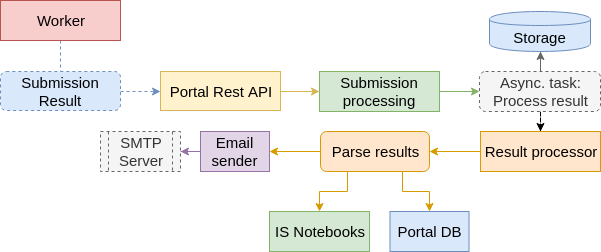
\includegraphics[width=\textwidth]{imgs/process-result.png}
  \end{center}
    \caption{Diagram spracovania výsledku}
    \label{fig:proc-result}
\end{figure}

\chapter{Implementácia komponentov systému}

Táto kapitola popisuje implementačné detaily systému a jednotlivých komponentov. Hlavnými spracovávanými komponentmi sú \emph{Pracovník} a \emph{testovací rámec KTDK}. Kapitola tiež približuje potrebné zmeny v~existujúcej implementácii Portálu potrebné na integráciu s~Pracovníkom a ostatnými službami.

Implementácia systému neodráža celý návrh z~dôvodu jeho rozsiahlosti a komplexnosti. Niektoré chýbajúce časti budú implementované ako samostatné bakalárske alebo diplomové práce, poprípade ako dobrovoľnícka činnosť jednotlivcov. Pre účely testovacej prevádzky boli niektoré potrebné časti nahradené zjednodušenou implementáciou, ktorá slúži ako prototyp a bude ju neskôr potrebné nahradiť plnou implementáciou.


\section{Implementácia Portálu}
\label{impl-portal}

Návrh a prvotná implementácia Portálu je popísaná v~bakalárskej práci Bc. Barbory Kompišovej, ktorá sa venuje hlavne problému autentizácie, vzťahom medzi entitami systému, ich správe a návrhu rozhrania\cite{kontr-portal}. Implementácia využíva jazyk Python verzie 3.6. 

\subsection{Štruktúra Portálu}

Hlavnou úlohou Portálu je poskytnúť organizačnú štruktúru a možnosť správy odovzdaní. Základné časti Portálu sú preto hierarchia entít, súbory potrebné na spracovanie odovzdaní a REST rozhranie poskytované webovou aplikáciou implementovanou pomocou mikrorámca \emph{Flask\footurl{http://flask.pocoo.org/}} a jeho rozšírení. 

Portál pracuje s~dvoma typmi dát:
\begin{itemize}
  \item \textbf{Entity systému} Portál ukladá v~relačnej databáze \emph{PostgreSQL}\footnote{\url{https://www.postgresql.org/}}, s~ktorou komunikuje pomocou \emph{ORM nástroja SQLAlchemy}\footurl{https://www.sqlalchemy.org/}, umožňujúceho zápis databázových dotazov pomocou konštruktov jazyka Python.
  \item \textbf{Súbory} ukladá na disk pomocou vlastnej knižnice \emph{storage}\footurl{https://gitlab.fi.muni.cz/grp-kontr2/kontr-storage-module}, abstrahujúcej prácu so súborovým systémom. Knižnica zabezpečuje získanie dát, ich spracovanie a následné uloženie.
\end{itemize}

\subsection{Zmeny oproti pôvodnej implementácii}

Zmeny potrebné pre integráciu s~Pracovníkom a testovaciu prevádzku sa týkali predovšetkým asynchrónneho spracovania odovzdaní, ktoré bolo v~pôvodnej verzii umožňovalo len uloženie odovzdania do Úložiska, už nie jeho ďalšie spracovanie. Ďalej bolo Portál potrebné integrovať s~fakultnou LDAP databázou, implementovať autentizáciu pomocou \emph{tajomstva (secret)} pre integráciu s~Pracovníkom, pozmeniť rozhranie a uľahčiť konfiguráciu a nasadenie Portálu.

\ssubsection{Asynchrónne spracovanie odovzdania}
\label{impl-portal-async}
Pre testovaciu prevádzku systému Kontr 2 bolo potrebné dokončiť všetky akcie potrebné na spracovanie odovzdania po jeho prijatí: jeho uloženie do Úložiska, získanie testovacích súborov a následné naplánovanie a odoslanie odovzdania Pracovníkovi. Ďalej bolo ako asynchrónnu úlohu potrebné implementovať spracovanie výsledku odovzdania, ktoré sa spúšťa po prijatí výsledku od Pracovníka. Implementácia plánovača ani nástroja na spracovanie odovzdania nie je súčasťou tejto práce, preto sú obe časti dodané v~zjednodušenej verzii --  plánovač používa fixný interval, počas ktorého je možné odovzdanie zrušiť a vyberá náhodného Pracovníka, spracovanie odovzdania nie je konfigurovateľné.

Nástroj pre asynchrónne spracovanie použitý v~Portále sa volá \emph{Celery}\footurl{http://www.celeryproject.org/}, ktorý implementuje logiku pre synchronizáciu dát a správu procesov, ktoré vykonávajú asynchrónne úlohy. 

Jednou z~výhod nástroja je možnosť pozdržať vykonávanie úlohy, čo zjednoduší plánovanie (implementáciu tzv. \emph{cancellation period}). Druhou zaujímavou možnosťou je periodické vykonávanie úloh pomocou \emph{celery-beat}, užitočné napríklad na pravidelnú kontrolu chýb spracovania odovzdania alebo čistenie systému.

Producentom úloh je časť aplikácie, ktorá beží ako REST API tzv. \emph{prijímač (listener)}, konzumentmi sú samostatné procesy, tzv. \emph{Celery pracovníci (Celery worker)}. Prijímač je v~kontexte Celery klientom, ktorý vkladá do úlohy do distribuovaného frontu úloh. Celery pracovník z~frontu úlohy postupne číta a spracováva. Štandardnou praxou je, že klient a pracovník zdieľajú kódovú základňu, vďaka čomu má pracovník prístup k~zdrojom klienta, napríklad databázovému spojeniu\cite{celery-intro}.

Ako \emph{message broker} bol použitý \emph{Redis (Remote Dictionary Server)}\footurl{https://redis.io/}, distribuované dátové úložisko typu kľúč-hodnota, uchovávané v~operačnej pamäti. Podporuje viacero dátových typov (reťazce, čísla, množiny, asociatívne polia, polia a pod.). Jednotlivé asynchrónne úlohy ukladá ako kľúče, hodnoty sú dodatočné informácie o~úlohe, napríklad jej parametre. Redis bude neskôr využitý aj v~plánovači a to na uchovávanie dodatočných informácií o~jednotlivých Pracovníkoch.

\begin{figure}[!ht]
  \begin{center}
    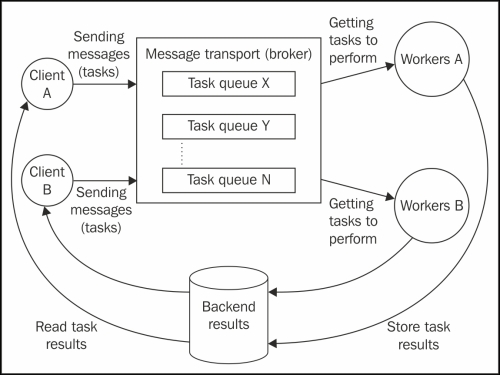
\includegraphics[width=\textwidth]{imgs/celery-arch.jpg}
  \end{center}
    \caption{Architektúra Celery\cite{celery-arch}}
    \label{fig:celery-arch}
\end{figure}

\ssubsection{LDAP}
Pre získanie atribútu užívateľa \emph{UČO} z~fakultného LDAP serveru bolo potrebné vytvoriť modul zapuzdrujúci komunikáciu s~týmto LDAP serverom. Modul využíva knižnicu \emph{ldap3}\footurl{https://ldap3.readthedocs.io/}. Využitie tejto integrácie je voliteľné a zapína sa nastavením url pre LDAP server. Dôvodom je predovšetkým to, že komunikácia s~LDAP serverom FI MU je možná len v~rámci fakultnej siete, takže inštancie Portálu bežiace mimo nej LDAP využívať nemôžu.

\ssubsection{Autentizácia pomocou tajomstiev}

Autentizácia pomocou \emph{tajomstiev (secretov)} bola v~pôvodnej implementácii dostupná len pre Pracovníkov, pričom pre Pracovníka bolo možné vygenerovať len jedno tajomstvo. Pomocou dedičnosti bol predstavený spoločný potomok pre entity \emph{User} a \emph{Worker} -- \emph{Client}. Na entitu Client bolo naviazané členstvo v~kurze pomocou entity \emph{Role} a kolekcia tajomstiev. Každý klient môže mať definovaných niekoľko tajomstiev, pre ktoré je možné nastaviť rôzne doby expirácie. Tajomstvá sú automaticky generované a v~databáze sú uložené v~hashovanej podobe rovnako ako heslá užívateľov.

Výhodou tajomstiev je možnosť ich využitia v~automatizovanmých skriptoch alebo externých nástrojoch, ktoré by inak vyžadovali manuálne zadané alebo uložené heslo užívateľa, čo z~bezpečnostných dôvodov nie je vhodné. Autentizácia pomocou tajomstva je doporučenou metódou autentizácie pomocou nástroja \emph{kontrctl}\footnote{\fullref{impl-other-parts}}.

\ssubsection{Ostatné zmeny}
Pre jednoduchšie načítavanie konfigurácie a zjednotenie s~ostatnými nástrojmi som použil knižnicu \emph{python-dotenv}, pomocou ktorej je možné prepísať premenné prostredia v~súbore \texttt{.env}. Táto zmena následne uľahčila nasadenie celého projektu. Medzi menšie zmeny, ktoré bolo potrebné spraviť, bolo nahradenie knižnice \emph{flask-restful}, knižnicou \emph{flask-restplus}\footurl{https://flask-restplus.readthedocs.io/en/0.12.1/}, ktorá podporuje generovanie \emph{swagger}\emph{https://swagger.io/specification/} dokumentácie pre REST API a úprava rozhrania Portálu pridaním nových koncových bodov.

\subsection{Administračný CLI Nástroj}

Na uľahčenie administrácie Portálu bol implementovaný konzolový nástroj umožňujúci priamu prácu s~Portálom. Využíva jednoduché rozšírenie \emph{Flask CLI}\footnote{\url{http://flask.pocoo.org/docs/1.0/cli/}} rámca Flask, ktoré využíva knižnicu \emph{click}\footurl{https://click.palletsprojects.com/en/7.x/}. 

CLI nástroj má prístup k~celému kontextu Portálu a jeho úlohou je umožniť jeho jednoduchú manuálnu správu a spúšťanie administračných skriptov. Nástroj Flask CLI, Portál používa aj na generovanie alebo aplikovanie databázových migrácii, pomocou ktorých je možné za behu meniť schému databázy. Okrem administrátorov smú nástroj používať aj bežní užívatelia Portálu. Autentizáciu a autorizáciu nástroj deleguje na Portál, umožnené je prihlásenie pomocou mena a hesla alebo mena a tajomstva.

\section{Implementácia Pracovníka}

Pracovník bol implementovaný ako webová aplikácia s~REST rozhraním podobne ako Portál. Jazykom implementácie je Python vo verzii 3.6. Rozhranie Pracovníka aj metódy autentizácie sú jednoduchšie než v~Portáli, podstatná časť je samotné spracovanie odovzdania.

Pracovník vystavuje REST rozhranie pomocou mikrorámca \emph{Flask} a jeho rozšírení. Autentizácia príchodzích požiadaviek pre Pracovníka je zaručená pomocou pevne definovaného \emph{tokenu}, ktorý musí byť súčasťou každého dotazu na Pracovníka v~autorizačnej hlavičke (\texttt{Authorization: Bearer <token>}). Toto zabezpečenie je možné rozšíriť o~klientskú autentizáciu pomocou verejného \emph{SSL certifikátu}\footurl{https://tools.ietf.org/html/rfc5246}, ktoré umožňuje vzájomnú autentizáciu serveru a klienta. 

Pracovník na spracovanie dlhotrvajúcich úloh používa nástroj Celery a Redis ako message broker. Celery klientom je tu opäť webová aplikácia, Celery pracovníkov Pracovník využíva viacero. (Viď časti \fullref{impl-portal-async} a \fullref{design-async-process})

Inštancia databázy Redis v~Pracovníkovi slúži okrem dočasného ukladania úloh pre Celery pracovníkov aj na uchovávanie stavu Pracovníka, napr. identifikátorov spracovávaných odovzdaní a aktuálnych verzii Docker obrazov. REST rozhranie a Celery pracovníkov je možné naškálovať na niekoľko súbežných procesov pomocou konfigurácie. Dáta v~Pracovníkovi sa rýchlo menia a nie je potrebné ich dlhodobo uchovávať, preto Redis ako databáza postačuje a nie je potrebné pridávať ďalšiu relačnú databázu.

\subsection{Kontajnerizačná technológia -- Docker}

Ako kontanjerizačná technológia bol použitý produkt \emph{Docker}. Bližšie informácie sa nachádzajú v~časti v~\fullref{design-worker-lc}

Pracovník zostavuje Docker obrazy z~aktuálnej verzie testovacích súborov automaticky pri každej ich zmene. Nutnou súčasťou testovacích súborov je \texttt{Dockerfile}\footurl{https://docs.docker.com/engine/reference/builder/} popisujúci inštrukcie potrebné k~zostaveniu konkrétneho obrazu.

Do projektu bola podpora pre \emph{Docker} pridaná pomocou oficiálnej knižnice \emph{docker-py}\footurl{https://docker-py.readthedocs.io/en/stable/}, ktorá obaľuje volania Docker príkazov do metód.

\subsection{Spracovanie odovzdania}

Pracovník po prijatí požiadavky na spracovanie nového odovzdania extrahuje všetky potrebné informácie a uloží ich do Redis-u. Následne vytvára asynchrónnu úlohu pre Celery pracovníka, v~ktorej sa spracovanie bude vykonávať.

Asynchrónna úloha najskôr skontroluje, či Pracovník obsahuje aktuálnu verziu testovacích súborov. To je možné zistiť pomocou ich \emph{odtlačku}, štandardne \emph{hash git commitu}, ktorý je súčasťou požiadavky na spracovanie odovzdania. Odtlačok testovacím súborom priraďuje Portál a ukladá ho v~svojej databáze. Pracovník má uložený zoznam aktuálnych odtlačkov pre rôzne projekty a v~prípade, že sa nový odtlačok nezhoduje s~uloženým alebo pre daný projekt zatiaľ neexistuje záznam dôjde k~stiahnutiu testovacích súborov, zostaveniu testovacieho obrazu a uloženiu nového odtlačku do databázy Pracovníka. 

Po ukončení prípravy testovacích súborov Pracovník stiahne študentovo odovzdanie a rozbalí ho do adresára unikátneho pre odovzdanie. Spolu s~ním vytvorí aj priečinok na uloženie výsledkov testovania. 

Následne dôjde k~vytvoreniu nového kontajneru, do ktorého sú oba priečinky pripojené (\emph{mount}) -- študentovo odovzdanie len s~oprávneniami pre čítanie, adresár na výsledky aj s~oprávnením pre zápis. Kontajner je vytvorený bez sieťového rozhrania, aby sa pre zvýšenie bezpečnosti zabránilo sieťovej komunikácii.

Kontajner je spustený s~minimálnymi možnými oprávneniami a s~právami užívateľa, pod ktorým beží Pracovník, vďaka čomu dochádza k~zvýšeniu bezpečnosti\footnote{Bez explicitného nastavenia sú kontajnery spúšťané s~právami užívateľa \emph{root}, čo predstavuje bezpečnostné riziko.}. Zároveň tak Pracovník môže bez problémov manipulovať so všetkými výsledkami vytvorenými počas behu kontajnera.

Po dokončení testovacieho procesu Pracovník skomprimuje priečinok s~výsledkami do jedného \emph{zip archívu}, ktorý odošle Portálu. Následne vyčistí prostredie, zmaže vytvorené priečinky a súbory, odstráni Docker kontajner a odstráni odovzdanie zo zoznamu aktuálne spracovávaných odovzdaní.

Pracovník je ľahko rozšíriteľný pre natívne vykonávanie odovzdaní, tzn. bez použitia kontajnerizačnej technológie Docker alebo jej nahradenie inou kontajnerizačnou technológiou.

\subsection{Administračný CLI Nástroj}

Rovnako ako Portál poskytuje Pracovník jednoduchý konzolový nástroj pomocou rozšírenia Flask CLI. Nástroj má prístup k~celému kontextu Pracovníka a obsahuje administračné príkazy, pomocou ktorých je možné vykonávať operácie, napríklad zistiť jeho stav, zaregistrovať ho do Portálu, alebo manuálne spustiť spracovanie odovzdania.

\section{Implementácia testovacieho rámca KTDK}

Testovací rámec KTDK je univerzálny testovací rámec, implementovaný v~jazyku Python 3.6. Súčasťou rámca je aj \emph{CLI nástroj} na vykonávanie testovacích scenárov a získavanie dodatočných informácií o~štruktúre scenárov, implementovaný pomocou knižnice \emph{click}.

\subsection{Konfigurácia}
Konfigurácia testovacieho rámca obsahuje statické informácie, ktoré sú potrebné pre jeho beh. Medzi konfiguračné parametre patria cesty k~potrebným adresárom (napr. pre testovacie súbory, odovzdania, výsledky), východzie parametre pre jednotlivé aplikácie a programy (prekladač, valgrind), nastavenie behu testov (časové limity, vývojársky mód). Všetky dostupné konfiguračné parametre je možné aj s~popisom nájsť v~dokumentácii nástroja \emph{KTDK}\footnote{\url{https://gitlab.fi.muni.cz/grp-kontr2/kontr-documentation/blob/master/ktdk/configuration.adoc}}.

Jednotlivé parametre potrebné pre beh testov je možné nastaviť pomocou príkazového riadka, premenných prostredia alebo ich prepísaním v~konfiguračnom súbore. Východzie hodnoty sa nachádzajú v~\emph{YAML} súbore \texttt{ktdk/resources/config/defaults.yml}. Tento súbor má najnižšiu prioritu, parametre nastavené ostatnými spôsobmi tieto hodnoty prepisujú.

Po načítaní a spustení vykonávania testovacích scenárov je konfigurácia jednotlivým \emph{úlohám a testom} prístupná pomocou objektu \emph{kontext}.


\subsection{Implementácia entít}

Dve základné entity slúžiace na popis testovacích scenárov v~KTDK sú \emph{Test} a \emph{Task (úloha)}. Oba sú objekty, ktorým je pri popise scenára možné pomocou konštruktora nastaviť parametre potrebné na ich identifikáciu. 

\texttt{Task} (úloha) je objekt, ktorému je potrebné implementovať \emph{protected} metódu \texttt{\_run}, ktorá je volaná pri procese spracovania úlohy.

Spustenie testov a úloh je zabezpečené pomocou tzv. \emph{spúšťača} (\emph{Runner}), ktorý definuje, v~akom poradí a akým spôsobom dôjde k~spusteniu jednotlivých úloh a testov. Každý test a úloha môže využívať iný spúšťač. Existujú východzie implementácie spúšťača, ktoré vykonávajú úlohy sekvenčne. V~budúcnosti by bolo možné implementovať paralelnú variantu, ktorá by mohla časť testov vykonávať súčasne. Poradie spúšťania definované dodanými spúšťačmi je priblížené v~časti \fullref{design-struct-test-scenarios}.

Inštancia spúšťača pre danú úlohu alebo test sa vytvára pri začatí ich spracovania. Spúšťač testu skontroluje podmienky pre beh testu, napríklad štítky, a v~prípade, že test nemá byť spustený, nastaví výsledok testu na preskočený. Inak pokračuje spustením úloh a dcérskych testov v~definovanom poradí.

Spúšťač nad úlohou volá metódu \texttt{invoke}, vykonávanú v~\emph{try-catch} bloku, v ktorom sú očakávané výnimky \texttt{RequireFailedError} a všeobecná \texttt{Exception}. Prvá z~nich nastáva, ak zlyhal \emph{require assert}, ktorý hovorí, že ak je ním testovaná podmienka vyhodnotená na \texttt{False}, má sa ukončiť vykonávanie testu a výsledok testu je vyhodnotený ako \texttt{FAIL}. Zachytenie všeobecnej výnimky znamená neočakávanú chybu -- chybný stav testovacieho rámca samotného. Výsledok testu je preto nastavený ako \texttt{ERROR} a mal by byť ďalej spracovaný administrátormi a vývojármi systému.

\subsection{Definícia testovacích scenárov}

Testovacie scenáre pre automatizované testovanie je možné pridať do repozitára s~testovacími súbormi do priečinka \texttt{kontr\_tests}. Z~tejto zložky KTDK načítava súbor \texttt{instructions.py}. Rámec je možné nastaviť aj na inú cestu k~súboru s~inštrukciami. Celý priečinok \texttt{kontr\_tests} je pridaný na štandardné cesty modulov jazyka Python\footnote{\url{https://docs.python.org/3/reference/import.html}}, čo zabezpečí, že všetky moduly a balíky definované v~tomto priečinku sú sprístupnené spúšťaciemu skriptu.

Príklady testovacích scenárov a inštrukcie na ich písanie je možné nájsť v~dokumentácii\footnote{\url{https://gitlab.fi.muni.cz/grp-kontr2/kontr-documentation/blob/master/ktdk/writing_scenarios_in_ktdk.adoc}} a repozitároch s~príkladmi\footnote{\url{https://gitlab.fi.muni.cz/grp-kontr2/examples/}}. 

\subsection{Spracovanie štítkov}

Každý test môže byť označený množinou štítkov(\emph{tags}), na základe ktorých je možné vybrať, ktoré majú byť spustené. Filtrovanie na základe štítkov vyžaduje, aby testy boli označené množinou štítkov a \emph{filtrovací výraz} predaný \emph{ktdk} pri spustení testovacích scenárov. Jedným z~riešených problémov bol formát výrazu, ktorý musel mať dostatočnú vyjadrovaciu silu, ďalším bol spôsob, ako tento formát vyhodnotiť. 

Prvotná implementácia používala ako vyhodnocovaný výraz zoznam štítkov a ich negácii, vyjadrených znakom \texttt{!}. Aby bol test spustený, musel obsahovať aspoň jeden pozitívny štítok z~výrazu a zároveň nesmel obsahovať žiadne negované.

Po preskúmaní možností a vyjadrovacej sily tejto implementácie bol ale zvolený iný variant, pomocou ktorého je možné spracovávať kompletné logické výrazy.

Príkladom je výraz \texttt{"naostro and not stylecheck"}, ktorý explicitne hovorí že musia byť splnené obe podmienky. Pohodlným rozšírením je umožnenie definovanie priority vyhodnotenia pomocou zátvoriek, ktoré zjednodušuje písanie komplexných výrazov. Tento spôsob je inšpirovaný metódou vyhodnocovania štítkov (\emph{markers}), ktorú používa testovací rámec \emph{pytest}\footurl{https://docs.pytest.org/en/latest/example/markers.html}.

Druhý variant je vyhodnocovaný pomocou interpretéra jazyka Python funkciou \texttt{eval}\footurl{https://docs.python.org/3.6/library/functions.html\#eval}. Vzhľadom na to, že funkcia \texttt{eval} je pri umožnení užívateľského vstupu potenciálne nebezpečná, bolo potrebné definovať, ku ktorým objektom, modulom a premenným má počas vyhodnocovania prístup, a následne do nej vložiť kontext, nad ktorým môže operovať. Implementácia interpretéra štítkov odstraňuje volaniu funkcie \texttt{eval} všetky dostupné globálne a lokálne objekty a nahradzuje ich kontextom, v~ktorom je každý štítok premenná nadobúdajúca hodnotu \emph{True} alebo \emph{False} na základe toho, či je na danom teste štítok definovaný. 

\section{Implementácia ostatných častí}

\label{impl-other-parts}
Súčasťou tejto práce bola implementácia ďalších, podporných projektov uľahčujúcich prácu s~hlavnými komponentmi systému a ich testovanie.

Knižnica \textbf{kontr-api} v~jazyku Python zaobaľuje REST-ové volania rozhrania Portálu do sady metód a odpovede na ne do objektov. Knižnica umožňuje autentizáciu voči Portálu a vykonávanie požiadaviek na Portál, ktoré realizuje knižnicou \emph{requests}\footurl{http://docs.python-requests.org/en/master/}. Knižnicu v~súčasnosti využívajú Pracovník a kontrctl. 

\textbf{Kontrctl} je konzolový nástroj využívajúci knižnicu \emph{click} na prijímanie a spracovanie príkazov a \emph{tabulate}\footurl{https://pypi.org/project/tabulate/} na štrukturované zobrazovanie tabuliek. Nástroj implementuje predovšetkým \emph{CRUD} operácie nad entitami Portálu cez kontr-api. Ďalej je pomocou neho možné spravovať viacero inštancii Kontru 2, ktoré sú rozlíšené pomocou tzv. \emph{remote}, predstavujúcich konfiguráciu inštancie pre kontrctl.

Pre každú spravovanú inštanciu je možné definovať vlastnú sadu parametrov a premenných, napríklad užívateľa, pod ktorým sa majú príkazy vykonávať, prístupové informácie \emph{(access\_token, refresh\_token, secret)}, \emph{URL}, na ktorej je dostupné rozhranie Portálu či východzie premenné. Informácie a konfigurácia pre jednotlivé \emph{remote} sa nachádza v~domovskom priečinku užívateľa v~zložke závislej na platforme\footnote{Pre linux je to: \texttt{~/.config/kontrctl/}, pre MS Windows: \emph{\%appdata\%/kontrctl}}.

Viac informácii o~\emph{kontrctl} obsahuje jeho dokumentácia\footnote{\url{https://gitlab.fi.muni.cz/grp-kontr2/kontr-documentation/tree/master/kontrctl}}.

\chapter{Nasadenie a popis prostredia}

Táto kapitola sa venuje možnostiam nasadenia systému ako celku vo vývojovom, testovacom a produkčnom prostredí. Súčasťou kapitoly je aj popis generovania výstupov vo forme knižníc a kontajnerov, pomocou ktorých je možné systém dodať.

Systém sa skladá z~viacerých repozitárov, ktoré je možné nájsť na fakultnom GitLabe\footnote{\url{https://gitlab.fi.muni.cz/grp-kontr2}}. Repozitáre obsahujúce výkonný kód majú nastavené \emph{CI/CD pipeline} pre automatickú kontrolu zdrojového kódu a spúšťanie testov nad každým \emph{merge requestom} do vetvy \emph{master}. Vďaka tejto automatizácii je možné čiastočne kontrolovať, či jednotlivé zmeny nespôsobia závady v~už existujúcom kóde komponentu.

\section{Nasadenie vývojovej verzie}

Nasadenie vývojovej verzie je možné dvoma základnými spôsobmi. Prvou z~nich je \emph{natívne nasadenie}, pre ktoré je potrebné stiahnuť si aktuálne verzie repozitárov jednotlivých projektov a nastaviť ich pomocou inštrukcii definovaných v~ich dokumentácii. Táto metóda vyžaduje inštaláciu a správne nastavenie všetkých závislostí na cieľovom stroji.

Druhou metódou je nasadenie pomocou kontajnerizačného nástroja \emph{Docker}. Pre každý komponent systému je definovaný Dockerfile popisujúci inštrukcie potrebné na zostavenie obrazu. Spustením obrazu vzniká kontajner obsahujúci danú komponentu a všetky jej závislosti. Zostavené \emph{obrazy} je možné nájsť v~docker registri \emph{(Docker~Hub)}\footnote{\url{https://hub.docker.com/u/kontr2}}. Obrazy je možné z~registra stiahnuť pomocou príkazu \texttt{docker pull <meno-obrazu>}.

Systém pozostáva zo siedmich kontajnerov \emph{(portal-gunicorn, portal-celery, worker-gunicorn, worker-celery, redis, postgres, frontend)}, medzi ktorými je potrebné vytvoriť prepojenia, spustiť ich so správnymi oprávneniami a pridať do nich \emph{persistent volumes} na správne destinácie. Pre zjednodušenie nastavenia a prepojenia častí bol vytvorený \emph{docker-compose súbor}\footnote{\url{https://docs.docker.com/compose/compose-file/}}, ktorý je vstupom pre nástroj slúžiaci na správu viacerých kontajnerov a zdrojov na jednom užívatelskom stroji \emph{docker-compose}\footnote{\url{https://docs.docker.com/compose/reference/}}. Nástroj umožnuje nasadiť celý systém pomocou troch príkazov\footnote{\texttt{docker-compose down \&\& docker-compose build \&\& docker-compose up}}. Táto metóda umožňuje jednoduché nasadenie systému pri vývoji, robí systém dostupnejším pre nových vývojárov a zjednodušuje nasadenie testovacej inštancie. Skript aj s~inštrukciami je možné nájsť v~pomocnom repozitári \emph{docker} \footurl{https://gitlab.fi.muni.cz/grp-kontr2/docker/tree/master/platform}.

Proces nasadenia vývojovej verzie pozostáva z~troch fáz. Prvou z~nich je získanie potrebných repozitárov, z~ktorých je systém zostavený: \emph{(Portál, Pracovník, Frontend a docker)}. Všetky repozitáre je potrebné stiahnuť pomocou verzovacieho nástroja Git. Druhou fázou je zostavenie obrazov z~aktuálnych verzii repozitárov. Treťou je inicializácia dát a vývojárskeho prostredia, ktorá zahŕňa vytvorenie databázových tabuliek a vloženie testovacích dát a entít do systému. Jedným z~krokov je aj inicializácia a zaregistrovanie Pracovníka do systému, čim je zabezpečené, že je systém po spustení pripravený na spracovávanie testovacích odovzdaní.

Výhodou kontajnerizacie celého systému je možné neskoršie nasadenie do systému pre automatické nasadenie, škálovanie a manažment kontajnerizovaných aplikácii. Možnosťami takéhoto nasadenia je napríklad \emph{docker swarm}\footnote{\url{https://docs.docker.com/engine/swarm/}} alebo \emph{kubernetes}\footnote{\url{https://kubernetes.io}}. FI MU uvažuje o~možnosti nasadenia niektorých svojich služieb, medzi ktoré by Kontr 2 mohol v~budúcnosti patriť, na Kubernetes cluster. 

\section{Nasadenie produkčnej verzie}
\label{deploy-prod}

Produkčná verzia je aktuálne nasadená v~službe \emph{Stratus.FI}\footnote{\url{https://stratus.fi.muni.cz/}}, privátnom cloude pre užívateľov z~FI MU postavenom na software \emph{OpenNebula}\footnote{\url{http://www.opennebula.org/}}.
Primárnym účelom je poskytnúť užívateľom prostredie na experimentovanie a rýchle vyskúšanie alebo aj produkčné použitie softvéru, ktorý z~rôznych dôvodov nemôže byť nainštalovaný priamo na serveroch spravovaných CVT FI, napríklad Anxur alebo Aisa\cite{fi-tech-stratus}.

Produkčné nasadanie pozostáva z~dvoch virtuálnych strojov. Na prvom beží backend a frontend Portálu a na druhom Pracovník. Oba stroje sú postavené na distribúcii CentOS\footurl{https://www.centos.org} vo verzii 7.5.

Systém využíva \emph{PostgreSQL} databázu dodávanú Fakultou informatiky pre študentské projekty ale aj služby bežiace na fakultnej infraštruktúre (napríklad GitLab). Výhodou tejto databázovej inštancie sú pravidelné zálohy a podpora zo strany CVT FI.

\begin{figure}[!ht]
  \begin{center}
    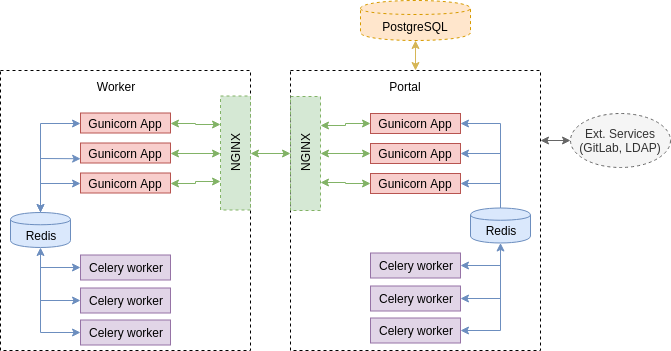
\includegraphics[width=\textwidth]{imgs/sys-deploy.png}
  \end{center}
    \caption{Schéma produkčného nasadenia systému}
    \label{fig:prod-deploy}
\end{figure}

\subsection{Produkčné nasadenie Portálu}

\begin{table}[h]
\begin{tabular}{l l}
Komponent & Veľkosť \\ [0.5ex] 
\hline
Operačná pamäť & 4GB  \\
Procesor & 4 virtuálne jadrá  \\
Veľkosť pevného disku&  50GB \\
\end{tabular}

\caption{Parametre virtuálneho stroja s~nasadeným Portálom} \label{tab:machine-portal}

\end{table}

Virtuálny stroj \emph{(viď \ref{tab:machine-portal})}, na ktorom je nainštalovaný Portál je dostupný z~verejnej siete a má pridelenú verejnú IP adresu a doménu \texttt{\url{https://kontr.fi.muni.cz}}. Pre doménu je vygenerovaný a podpísaný certifikát od certifikačnej autority \emph{Let's encrypt}\footnote{\url{https://letsencrypt.org/}}. Využitie protokolu \emph{HTTPS}\cite{RFC2818} postaveného nad TLS\cite{RFC8446} zabezpečuje šifrovanú komunikáciu medzi Portálom (serverom) a jednotlivými klientmi (Pracovník, Frontend, kontr-api).

Konfigurácia HTTPS spojenia, sprístupnenie rozhrania Portálu a Frontendu nástroja Kontr bolo dosiahnuté pomocou \textit{NGINX}\footnote{\url{https://www.nginx.com/resources/wiki/}} HTTP servera a \emph{reverse proxy}. Backend Portálu je spustený v~niekoľkých inštanciách (procesoch) pomocou Python WSGI HTTP serveru \emph{Gunicorn}\footurl{https://gunicorn.org/}. NGINX je nastavená ako proxy, slúži ako verejné rozhranie a všetky požiadavky na rozhranie Portálu sú posielané cez ňu. Rovnako NGINX sprístupňuje aj statický obsah (Frontend), zložený z~HTML, Typescript, css súborov a obrázkov.

Gunicorn a Celery bežia ako samostatné služby obsluhované pomocou \texttt{systemd}. Bolo pre ne nutné napísať vlastné \emph{servisné súbory}\footnote{\url{https://www.freedesktop.org/software/systemd/man/systemd.service.html}}. Komunikáciu pre asynchrónne spracovávanie služieb zabezpečuje služba Redis, dostupná len na lokálnej sieti stroja.

\subsection{Produkčné nasadenie Pracovníka}

\begin{table}[h]
\begin{tabular}{l l}
Komponenta & Veľkosť \\ [0.5ex] 
\hline
Operačná pamäť & 2GB  \\
Procesor & 2 virtuálne jadrá  \\
Veľkosť pevného disku&  20GB \\
\end{tabular}
\caption{Parametre virtuálneho stroja s~nasadeným Pracovníkom} \label{tab:machine-worker}
\end{table}

Virtuálny stroj \emph{(viď \ref{tab:machine-worker})}, na ktorom je nainštalovaný Pracovník, sa nachádza na privátnej sieti Stratus.FI a nie je dostupný mimo fakultnej siete. Pracovník a Portál spolu komunikujú cez privátnu sieť, pretože Pracovník kvôli nastaveniu firewallu nemôže komunikovať s~Portálom po verejnej sieti. Nanešťastie to spôsobuje problémy s~validáciou certifikátu vydaného pre Portál, preto bolo potrebné zmeniť v~\texttt{/etc/hosts} súbore vyhodnotenú IP adresu Portálu na privátnu IP adresu, z~ktorej je Portál dostupný na privátnej sieti.

Na Pracovníkovi je nasadený NGINX, pomocou ktorého je zabezpečené rozhranie Pracovníka pomocou \emph{SSL/TLS self-signed certifikátu}, ktorý bol podpísaný zdieľanou certifikačnou autoritou pre Portál a Pracovníka. Problémom tohoto riešenia bol fakt, že knižnica \emph{requests} má v~sebe vložený vlastný zoznam \emph{CA (Certifikačných autorít)}\cite{RFC5280} a ignoruje \emph{systémový trust store}. Našťastie je možné pomocou premennej prostredia prepísať cestu k~\emph{zoznamu CA (CA bundle)}.

Rovnako ako pre Portál bolo pre Pracovníka potrebné vytvoriť servisné súbory pre \texttt{systemd} a nainštalovať a spustiť vlastnú inštanciu Redisu.

\subsection{Zabezpečenie pomocou SSL/TLS certifikátov}

Komunikáciu v~systéme je potrebné v~produkčnom prostredí zabezpečiť. REST rozhrania Portálu a Pracovníka boli zabezpečené pomocou SSL/TLS, vďaka ktorému komunikácia prebieha šifrovane. 

Pomocou SSL certifikátov je možné vyžadovať aj autentizáciu klienta voči serveru.
Pre časť operácii sa Pracovník správa ako klient voči Portálu a pre druhú časť naopak ako server, preto je potrebné, aby sa overovali obe strany komunikácie. Overenie vyžaduje certifikačnú autoritu, ktorá podpísala certifikát serveru aj klienta\cite{RFC2818}. Klient aj sever musia mať certifikačnú autoritu pridanú medzi \emph{trusted}. Nevýhodou tejto metódy je komplikovaná konfigurácia na strane serveru aj na strane klienta, ktorá pre menej skúseného administrátora môže predstavovať netriviálnu komplikáciu.

Súčasné nasadenie využíva len verifikáciu certifikátu serveru, klientský certifikát sa neoveruje.

\subsection{Automatizácia nasadenia}

V~budúcom vývoji je plánované automatizovať proces nasadenia celého systému v~podobe inštalátora, implementovaného napríklad v~podobe \emph{Ansible playbooks}. \emph{Ansible} je nástroj, ktorý automatizuje inštalovanie systému, konfiguráciu a nasadzovanie aplikácii\cite{ansible}. 

V~súčasnosti existuje repozitár s~\emph{Ansible playbookmi}\footnote{\url{https://gitlab.fi.muni.cz/grp-kontr2/ansible}} pre automatické nasadenie a aktualizáciu aplikácii bežiacich na produkčných strojoch. Playbook stiahne zmeny z~repozitárov v~Gitlabe, nainštaluje závislosti, spustí migrácie databázy, vygeneruje novú verziu Frontendu a reštartuje Gunicorn a Celery služby.

Pomocou tohoto skriptu je možné nasadzovať zmeny okamžite po tom, čo sú otestované, bez nutnosti zdĺhavo sa prihlasovať na server a manuálne vykonávať všetky príkazy. V~budúcom vývoji je v~pláne automatizovať celý proces ešte viac -- vždy po otestovaní a prebehnutí všetkých potrebných verifikácií spustiť tento skript automaticky, čím by každá zmena bola nasadená bez manuálneho zásahu.

\section{Balíčkovanie}

Súčasťou výstupov tejto práce sú tiež tri balíčky, dostupné na stránke \emph{PyPi}\footurl{https://pypi.org/} -- repozitár balíčkov tretích strán pre jazyk Python. Balíčky je možné vďaka tomu nainštalovať pomocou nástroja \emph{pip}\footurl{https://pypi.org/project/pip/} (viď \ref{tab:packages}).

Balíčky pri zostavovaní využívajú knižnicu \emph{setuptools}\footurl{https://pypi.org/project/setuptools/} a zostavovací skript \texttt{setup.py}, dostupný v~každom repozitári pre daný projekt.

Generovanie balíčkov je popísané v~oficiálnej dokumentácii \footurl{https://packaging.python.org/tutorials/packaging-projects/}, podľa ktorej boli balíčky zostavené. Výstupom procesu zostavenia sú archív s~dodanou implementáciou a \emph{wheel}\footurl{https://wheel.readthedocs.io/en/stable/} súbor metadátami o~balíčku. Tieto súbory sú následne nahrané do Python repozitára PyPi, pre nahranie bol použitý nástroj \emph{Twine}\footurl{https://pypi.org/project/twine/}. Odoslať balíčky do repozitáru môže len registrovaný užívateľ, preto bolo potrebné vytvoriť nového užívateľa, ktorý je aj správcom balíčkov.

\begin{table}[h]
\begin{tabular}{l l}
Meno balíčka & Príkaz na inštaláciu  \\ [0.5ex] 
\hline
\emph{ktdk}\footurl{https://pypi.org/project/ktdk/} & \texttt{pip install ktdk}  \\
\emph{kontr-api}\footurl{https://pypi.org/project/kontr-api/} & \texttt{pip install kontr-api}  \\
\emph{kontrctl}\footurl{https://pypi.org/project/kontrctl/} &  \texttt{pip install kontrctl} \\
\end{tabular}
\caption{Zoznam balíčkovaných projektov} \label{tab:packages}
\end{table}


\chapter{Testovacia prevádzka}

Testovacia prevádzka prebiehala v~obmedzenom režime vzhľadom na to, že systém stále nie je dokončený. Testovacie prostredie bolo predstavené v~časti \fullref{deploy-prod}. Testovanie bolo umožnené všetkým vyučujúcim predmetu PB161 a vybraným študentom. Študentov sa prihlásilo sedem a testovacia prevádzka prebiehala na úlohe \emph{HW03 (Bomberman)}. Pre účastníkov testovania bolo vytvorené interné diskusné fórum v~IS MU, v~ktorom mohli nahlasovať chyby, pýtať sa na nejasnosti alebo navrhovať rôzne vylepšenia systému.

Študenti odovzdávali svoje riešenia cez webové rozhranie Portálu (Frontend), v~ktorom si následne mohli prezrieť výsledky testovania (počet bodov a jednotlivé testy s~informáciou o~ich úspechu alebo neúspechu). Obmedzenia testovacej prevádzky boli napríklad chýbajúca integrácia \emph{review toolu}, plánovača a duplikovanie odovzdaní medzi novým a starým systémom Kontr, ktorá prebiehala manuálne. Študenti boli za testovanie a hľadanie chýb odmenení bonusovými bodmi.

\section{Výstup testovania}
Výstupmi testovania boli predovšetkým odhalené chyby a nedostatky systému a štatistiky využitia systému počas prevádzky.

\subsection{Chyby nájdené počas testovania}

Pred samotným študentským testovaním boli odhalené viaceré nedostatky v~\emph{logovaní udalostí} odohrávajúcich sa v~systéme. Hlavným nedostatkom bola nemožnosť priradenia aktéra k~danej udalosti, čo bolo potrebné pridať. Logy boli rozdelené do niekoľkých súborov zoskupujúcich logicky súvisiace oblasti, napríklad \emph{autorizačný log}, v~ktorom sa zaznamenáva len každý pokus o~prihlásenie.

Študentské testovanie odhalilo viacero chyb a nedostatkov vo Frontende systému. Pre väčšinu z~nich bola založená Issue v~GitLab repozitári projektu a časť z~nich sa už podarilo opraviť. Závažnejšie nájdené chyby sa týkali backendu a testovacieho rámca \emph{KTDK}. Sem patrilo nekorektné spracovanie odovzdania, nesprávne spočítanie bodov a chybné spracovanie asynchrónnych úloh.

Chyby týkajúce sa nesprávneho uloženia odovzdania a nesprávneho počítania bodov by už mali byť opravené. Problémom bol špecifický prípad, kedy test zlyhal na \texttt{SIGSEGV}\footnote{\url{http://man7.org/linux/man-pages/man7/signal.7.html}}, kedy vygenerovaný \emph{JUnit výstup}, ktorý je neskôr spracovávaný, nebol validný\footnote{Súbor bol nekompletný, čo bolo spôsobené nedokončením zápisu z~dôvodu ukončenia programu.}. Vzhľadom na to, že \emph{JUnit} výstup je generovaný testovacím rámcom \emph{Catch2}, bolo jediným riešením za test udeliť nulový počet bodov.

V~prípade chyby pri spracovaní asynchrónnej úlohy bolo chybu možné dohľadať v~logoch, no informácia o~nej sa nepremietla do žiadneho jej výstupu.

\subsection{Vybrané štatistiky}

Z~testovania úlohy HW03 (Bomberman) v~predmete PB161 v~semestri jeseň 2018 vzišli nasledujúce štatistiky.

\begin{table}[h]
\begin{tabular}{l l}
Počet testovacích odovzdaní & $31$  \\
Čas potrebný pre spracovanie s~\emph{docker-build}\footnote{Pri prvom odovzdaní so zmenenými testovacími súbormi je potrebné znovu zostaviť obraz} & $ \sim 5 min $ \\
Čas priemerný pre spracovanie odovzdania s~exist. obrazom & $\sim 2 min$\\
Dĺžka behu testovacích scenárov v~KTDK &  $\sim 85 s$ \\
\end{tabular}
\caption{Vybrane štatistiky pre spracovanie odovzdaní} \label{tab:proc-time-general}
\end{table}

Čas potrebný na spracovanie odovzdania bol počítaný od momentu vytvorenia odovzdania po uloženie výsledkov do Portálu.

Rozdiel časov vykonávania testov v~KTDK a pôvodnej implementácii Kontru je ovplyvnený iným spôsobom vykonávania testov. Jedným z~faktorov je, že samotné zostavenie v~Kontri 2 prebieha pomocou nástrojov \emph{cmake} a \emph{make} namiesto priameho volania prekladača.

Druhý ovplyvňujúci faktor je, že každý jeden test v~testovacom rámci \emph{Catch2} bol v~Kontri 2 spúšťaný a vyhodnocovaný samostatne -- implementácia extrahuje zoznam testov a následne ich vykonáva postupne ako samostatné procesy, ktoré vyhodnocuje zvlášť. Tým bolo možné docieliť, že pri páde jedného testu na chybnej práci s~pamäťou zlyhal iba tento test, nie celý testovací scenár. Testy pre starý Kontr spúšťali všetky testy ako jeden proces, čo znamenalo nižšiu réžiu a rýchlejšie vyhodnotenie.

\ssubsection{Spotreba diskového priestoru}

\begin{table}[h]
\begin{tabular}{l l l}
Meraná metrika & Reálna & Kompr. \\ [0.5ex] 
\hline
Celková veľkosť súborov v~úložisku &  $53MB$ & --  \\
Priemerná veľkosť zdroj. súborov pre odovzdanie & $308KB$ & $100KB$ \\
Priemerná veľkosť výsledkov pre odovzdanie & $500KB$ & $66 KB$ \\
Maximálna veľkosť výsledkov & $1.4MB$ &  $96KB$ \\
Veľkosť jedného odovzdania v~starom Kontri & $30MB$ & -- \\ 
\end{tabular}
\caption{Štatistiky spotreby miesta na disku pre odovzdania} \label{tab:storage-used}
\end{table}

Z~dát \emph{(viď \ref{tab:storage-used})} pre Kontr 2 vyplýva, že pre 1000 odovzdaní \emph{(100 študentov po 10 odovzdaní)} je potrebných $(500 KB + 308KB \approx 1MB) * 1000 \approx 1 GB$ miesta, v~prípade komprimovanej varianty je to $(66KB + 100KB \approx 200KB) * 1000 \approx 200MB$. Pre starý Kontr znamená 1000 odovzdaní v~nekomprimovanom stave spotrebu \emph{30GB}.

Jedno odovzdanie v~starom Kontri obsahuje zdrojové súbory, výsledky testovania ale aj zostavené binárne súbory, ktoré sa v~Kontri~2 nachádzajú v~priečinku \emph{workspace}, ktorá je po skončení testovania zahodená.
Miesto spotrebované nástrojom Kontr~2 je v~nekomprimovanej podobe 30-krát menšie než v~pôvodnom Kontri. Pre komprimovaný variant je spotreba miesta na disku pre Kontr~2 menšia 150-krát.

Jedným z~problémov Kontru je neustále prekračovanie kvóty na stroji Aisa, ktoré malo za následok zavedenie špeciálnych opatrení, ako napríklad obmedzenie maximálnej veľkosti študentských repozitárov. Pre Kontr 2 by na základe uvedených odhadov tento problém nemusel byť tak závažný.

\subsection{Jednoduché záťažové testy}

Testovacia inštancia prešla aj jednoduchými záťažovými testami, aby sa odhalili limity aktuálneho nasadenia. Namerané výsledky sú zobrazené v~tabuľke \ref{tab:timelimits}.
Uvedené dĺžky sú počítané ako rozdiel časov vytvorenia odovzdania a skončenia jeho vykonávania pre najdlhšie bežiace odovzdanie danej série.

\begin{table}[h]
\begin{tabular}{l l}
Počet súbežných odovzdaní & dĺžka vykonávania odovzdania  \\ [0.5ex] 
\hline
1 &  2 min  \\
2 & 3.5 min  \\
3 & 5 min \\
4 & 7.5 min \\  
5 & Odovzdania nedobehli v~časovom limite \\
\end{tabular}
\caption{Čas potrebný pre spracovanie $N$ odovzdaní} \label{tab:timelimits}

\end{table}

Päť súbežných odovzdaní spotrebovalo všetku dostupnú pamäť Pracovníka pri preklade súborov obsahujúcich testy. Štyri paralelné odovzdania predstavujú reálny limit pre danú úlohu. 

Problém je možné odstrániť pridaním ďalších prostriedkov, či už vo forme väčšieho limitu operačnej pamäte alebo dodatočnými Pracovníkmi.

Systém má v~súčasnosti obmedzenú kapacitu a používa sa naozaj len v~testovacej prevádzke, ale je navrhnutý tak, aby ho bolo možné ľahko preniesť na inú infraštruktúru a rozšíriť.

\chapter{Záver a budúci vývoj systému}
\addcontentsline{toc}{chapter}{Záver}

Úlohou práce bolo vypracovať analýzu a vysokoúrovňový návrh systému opravy domácich úloh Kontr 2 a implementáciu jeho podsystému pre spracovanie odovzdaní. 
Dôraz pri návrhu bol kladený na splnenie požadovaných prípadov užitia, zohľadnenie požiadaviek predmetov, ktoré by mali záujem systém používať a jeho ľahkú rozšíriteľnosť.

Systém ako celok bol rozdelený do nezávislých komponentov, koncipovaných ako samostatné aplikácie alebo moduly (knižnice), ktoré je možné v~prípade potreby nahradiť alebo rozšíriť. Nezávislosť komponentov vyžadovala jednoznačnú definíciu rozhraní a použitých komunikačných kanálov.

Návrh systému sa venuje predovšetkým vysokoúrovňovému pohľadu na systém a detailne rozpracováva iba malú podmnožinu navrhnutých komponentov. Podrobné priblíženie a implementácia jednotlivých častí systému, napríklad Portálu, je súčasťou iných prác.

V~kapitole venujúcej sa implementácii je priblížená implementácia podsystému pre spracovanie odovzdaní, integrácia s~existujúcim Portálom a zmeny, ktoré v~ňom bolo potrebné spraviť, a pomocné nástroje a knižnice potrebné pre uľahčenie práce so systémom.

Na implementačnú kapitolu nadväzuje kapitola predstavujúca možnosti nasadenia, ktorá detailne popisuje produkčné prostredie, stroje na ktorých je produkčná verzia nasadená. 

Posledná kapitola popisuje priebeh testovacej prevádzky, nájdené problémy, návrhy na vylepšenie a výstupy v~podobe štatistík využitia vybraných systémových prostriedkov a časov spracovania.

Výstupom tejto práce je systém schopný spracovať a vyhodnotiť odovzdanie, tvoriaci základ pre ďalšie rozširovanie a dopĺňanie funkcionality. Celý projekt je verejne dostupný a má otvorený zdrojový kód, preto ktokoľvek, kto má záujem, má možnosť prispievať a rozšíriť ho. So systémom sa stretne každý študent, ktorý si prejde základným kurzom nízkoúrovňového programovania, preto je možné týchto ľudí zaujať a dať im možnosť vyskúšať si prispieť do projektu s~otvoreným zdrojovým kódom. 
Nástroj by mohol mať úspech minimálne tým, že je implementovaný pomocou moderných technológii, je vyvíjaný priamo na FI MU a bude sa dotýkať väčšiny študentov.

Nadväzujúce práce by mali priniesť zásadnejšie zmeny a rozšírenia systému. Autor tejto práce plánuje na vytvorenom projekte ďalej pracovať a spravovať ho. V~systéme je ešte mnoho chýb a je potrebné pridať rozsiahlejšiu dokumentáciu a návody, ktoré by ukázali, ako so systémom pracovať a vysvetlili jednotlivé jeho časti.

Systém sa bez ďalších dobrovoľníkov nezaobíde, nielen kvôli potrebe vývoja nových rozšírení, ale hlavne jeho testovania, nasadenia a správe systému. Všetka táto \emph{skrytá} práca je pre beh celého systému nevyhnutná.


\appendix
\chapter{Elektronické prílohy}
Všetky relevantné repozitáre projektu Kontr 2.0 majú štítok: \texttt{v1.0}, ktorý zodpovedá odovzdanej verzii v~elektronickom archíve dodanom ako súčasť tejto práce.

Zoznam príloh zahrnutých v~elektr. archíve:

\begin{itemize} 
	\item Implementácia backendu Portálu
	\item Implementácia Pracovníka
	\item Implementácia KTDK
	\item Implementácia kontrctl
	\item Ansible playbook na aktualizáciu produkčtnej verzie
    \item Časť konfigurácie produkčného nasadenia systému. 
\end{itemize}

\chapter{Prehľad častí systému}

\hspace{\parindent}\textbf{Portál} -- Organizačná časť systému, tzv. Backend, ktorý poskytuje verejné API pre klientov.

\textbf{Úložisko} -- Modul Portálu slúžiaci na uchovávanie súborov súvisiacich s~odovzdaním -- odovzdané súbory, testovacie súbory a výsledky testovania.

\textbf{Nástroj na spracovanie odovzdania} -- Súčasť Portálu, zabezpečuje spracovanie odovzdania a jeho výsledkov, je možné v~ňom definovať akcie, ktoré sa majú vykonať pri prijatí nového odovzdania, ale aj po prijatí výsledkov.

\textbf{Prvý plánovač} -- Definuje kedy sa má odovzdanie vykonať a limity na počet odovzdaní užívateľa pre príslušný projekt.

\textbf{Druhý plánovač} -- Priraďuje odovzdania jednotlivým pracovníkom na základe ich vyťaženia a definovaných obmedzení.

\textbf{Pracovník} -- Zabezpečuje testovacie prostredie pre spúšťanie odovzdaní, ktoré mu predá Portál. Dodaná implementácia využíva kontajnerizačnú technológiu Docker.

\textbf{KTDK} -- Testovací rámec pre Kontr 2.0 implementovaný v~jazyku Python. Slúži na definíciu a vykonávanie testovacích scenárov.

\textbf{kontr-api} -- Knižnica pre jazyk Python, ktorá zaobaľuje REST API Portálu a sprostredkováva požadovanú funkcionalitu pomocou objektov a metód.

\textbf{kontrctl} -- CLI klient pre správu a komunikáciu s~portálom využívajúci kontr-api.

\textbf{Frontend} -- Single-Page aplikácia pre webové prehliadače napísaná v~rámci Angular.



\chapter{Zoznam technológii}

\hspace{\parindent}\textbf{Flask} -- Minimalistický webový rámec použitý na vytvorenie REST API pre Portál a Pracovníka.

\textbf{Gunicorn} -- Jednoduchý HTTP server pre Python aplikácie, používa ho Portál aj Pracovník na beh Flask REST API.

\textbf{SQLAlchemy} -- ORM databázová knižnica, ktorá zabezpečuje komunikáciu s~databázou a prevod databázových tabuliek do entít v~systéme.

\textbf{Celery} -- Nástroj na asynchrónne spracovávanie náročnejších úloh. Využíva ho Portál aj Pracovník.

\textbf{Redis} -- \emph{Message Broker}, databáza typu kľúč-hodnota v~operačnej pamäti. Je využívaná nástrojom Celery, ktorý pomocou neho buduje distribuovaný front úloh.

\textbf{Docker} -- Kontajnerizačná technológia umožňujúca spúšťanie aplikácii v~oddelenom prostredí, využívajúca vizualizáciu na úrovni OS. Docker je používaný Pracovníkom na vykonávanie odovzdaní a môže byť použitý pri nasadení vývojovej verzie.

\textbf{Click} -- Knižnica na písanie CLI aplikácii, použitá v~Portáli, Pracovníkovi, KTDK a Kontrctl.

\textbf{pytest} -- Rámec na písanie jednotkových aj integračných testov v~jazyku Python.

\textbf{requests} -- Knižnica na odosielanie a spracovanie HTTP požiadavkov, použitá v~\emph{kontr-api} a v~Portáli na komunikáciu s~Pracovníkom.

\textbf{Pipenv} -- Nástroj na správu závislostí a virtuálnych prostredí pre jazyk Python

\textbf{Ansible} -- Nástroj na automatizované spúšťanie príkazov a akcii na vzdialených strojoch. Používaný na aktualizáciu produkčnej verzie systému.

\textbf{Angular} -- Rámec na tvorbu frontend aplikácii.

\textbf{NGINX} -- HTTP Server, použitý ako proxy pre Portál a Pracovníka. Rieši zabezpečenie pomocou SSL/TLS certifikátov, sprostredkováva Frontend a preposiela požiadavky Gunicornu.

\textbf{Let's encrypt} -- Voľne dostupná certifikačná autorita, ktorá zdarma vystavuje SSL certifikáty. Bola využitá pri vystavení certifikátu pre doménu, na ktorej beží produkčná verzia Portálu.

\textbf{Setuptools} -- Knižnica na tvorbu balíčkov pre Python.

\textbf{Twine} -- Knižnica na nahranie balíčkov do PyPi repozitárov.

\textbf{Gitlab CI/CD} -- CI/CD Pipeline pre Gitlab, ktorá slúži na automatické spúštanie testov nad merge requestami a master vetvou celého projektu.

\textbf{Gitlab} -- Slúži ako jedna z~metód autentizácie užívateľov v~systéme. Spoločne s~LDAP-om sprístupňujú informácie o~užívateľoch.

\textbf{LDAP} -- Faklutná databáza s~dátami o~užívateľoch, ako napríklad ich UČO. Používaný Portálom pri vytváraní nových užívateľov.


\end{document}
